%
%\documentclass[onecolumn,traditabstract]{aa}  
\documentclass[twocolumn,traditabstract]{aa}  
\UseRawInputEncoding
%\pdfoutput=1
\usepackage{fixltx2e}
\usepackage[english]{babel}
\usepackage{graphicx,amsmath}
\usepackage{epstopdf}
\usepackage{epsf,color}
\usepackage[mathscr]{eucal}
\usepackage{amsmath}
\usepackage{amssymb,amsfonts}
\usepackage{natbib}
\usepackage{graphicx}
\usepackage{txfonts}
\usepackage{dsfont}
\definecolor{Mygreen}{rgb}{0.00, 0.5, 0.5}
\definecolor{Mypink}{rgb}{1.0, 0.0, 0.5}
\definecolor{Myblue}{rgb}{0.00, 0.2, 0.8}
\definecolor{Myred}{rgb}{0.80, 0.2, 0.0}
\usepackage[breaklinks, citecolor=Myblue, linkcolor=Mygreen, urlcolor=Mygreen, colorlinks=true, debug, baseurl=' ']{hyperref}
\usepackage{float}
\usepackage{color}
%\usepackage{siunitx}
%\usepackage{mathrsfs}

%\DeclareSIUnit\parsec{pc}
%\DeclareSIUnit\erg{erg}
%\DeclareSIUnit\deg{deg^{-2}}
%\DeclareSIUnit\count{cnt}

\def\intk#1{\displaystyle\int\frac{d^2k_{#1}}{(2\pi)^2}}
\def\intr#1{\displaystyle\int d^2r_{#1}}
\def\simlt{\lower.5ex\hbox{$\; \buildrel < \over \sim \;$}}
\def\simgt{\lower.5ex\hbox{$\; \buildrel > \over \sim \;$}}
\def\NIKA{\textit{NIKA}}
\def\Skydip{\textit{Skydip}}
\renewcommand{\arraystretch}{1.3}

\bibpunct{(}{)}{ and}{a}{}{,}
\bibliographystyle{aa}

%%%%%%%%%%%%%%%%%%%%%%%%%%%%%%%%%%%%%%%%
% Rexcess font
%\newfont{\gwpfont}{cmssqi8 scaled 1000}
\newfont{\gwpfont}{cmssq8 scaled 1000}
\newcommand{\rexcess}{{\gwpfont REXCESS}}
%%%%%%%%%%%%%%%%%%%%%%%%%%%%%%%%%%%%%%%%

\begin{document}

\def\aj{AJ}%
\def\araa{ARA\&A}%
\def\apj{ApJ}%
\def\apjl{ApJ}%
\def\apjs{ApJS}%
\def\aap{A\&A}%
 \def\aapr{A\&A~Rev.}%
\def\aaps{A\&AS}%
\def\mnras{MNRAS}
\def\ssr{SSRv}
\def\nat{Nature}
\def\jcap{JCAP}

\def\Mgv{M_{\rm g,500}}
\def\Mg{M_{\rm g}}
\def\YX {Y_{\rm X}}
\def\LXv {L_{\rm X,500}}
\def\TX {T_{\rm X}}
\def\fgv {f_{\rm g,500}}
\def\fg  {f_{\rm g}}
\def\kT {{\rm k}T}
\def\ne {n_{\rm e}}
\def\Mv {M_{\rm 500}}
\def \Rv {R_{500}}
\def\keV {\rm keV}
\def\Yv{Y_{500}}


\def\MT {$M$--$T_{\rm X}$}
\def\MYX {$M$--$Y_{\rm X}$}
\def\MMg {$M_{500}$--$M_{\rm g,500}$}
\def\MgT {$M_{\rm g,500}$--$T_{\rm X}$}
\def\MgY {$M_{\rm g,500}$--$Y_{\rm X}$}

\def\msol {{\rm M_{\odot}}}

\def\lesssim{\mathrel{\hbox{\rlap{\hbox{\lower4pt\hbox{$\sim$}}}\hbox{$<$}}}}
\def\gtrsim{\mathrel{\hbox{\rlap{\hbox{\lower4pt\hbox{$\sim$}}}\hbox{$>$}}}}

\def\psz{PSZ2\,G144.83$+$25.11}

% satellites
\def\xmm{XMM-{\it Newton}}
\def\planck{{\it Planck}} 
\def\chandra{{\it Chandra}}
\def \rosat {\hbox{\it ROSAT}}
\newcommand{\excpres}{{\gwpfont EXCPRES}}
\newcommand{\ma}[1]{\textcolor{red}{{ #1}}}
%###############################################################################################
%##########################              START THE PAPER             ##########################################
%###############################################################################################
\title{Simulation of the NIKA2 SZ large program with MUSIC clusters\\ I. Impact of ICM disturbances on the mean pressure profile}

\author{version 1.0}

\abstract {The accurate characterization of the shape, the intrinsic scatter and the redshift evolution of the mean pressure profile of galaxy clusters is essential to understand the large-scale structure formation processes. It will enable estimating the biases and systematic effects that currently prevent cosmological analyses based on thermal Sunyaev-Zel'dovich (tSZ) surveys to obtain precise cosmological constraints. This is one of the main goals of the on-going New IRAM Kids Arrays (NIKA2) SZ large program. This program aims at mapping the tSZ signal of a representative cluster sample selected from the \planck\ and ACT catalogs and spanning a redshift range $0.5 < z < 0.9$. We use the hydrodynamical N-body simulation \emph{Marenostrum MUltidark SImulations of galaxy Clusters} (MUSIC) in order to simulate realistic NIKA2 and \planck\ tSZ observations of MUSIC synthetic clusters selected using the same procedure used to define the NIKA2 SZ large program sample. The NIKA2 and \planck\ simulated maps are jointly analyzed in order to estimate the intracluster (ICM) pressure profile of each cluster. The comparison of the deprojected profiles with the true radial profiles extracted from the MUSIC simulation allows us to validate the NIKA2 SZ pipeline and to study the impact of ICM disturbances on the characterization of the ICM pressure distribution at high redshift. After normalizing each profile by the integrated quantities estimated under the hydrostatic equilibrium hypothesis, we estimate the mean pressure profile of the selected clusters and study the impact of the ICM dynamical state on both its slopes and associated scatter. The mean pressure profile estimated using the NIKA2 and \planck\ simulated maps is compatible with the one obtained directly from the simulation in the range of scales that can be recovered by NIKA2. We observe that the scatter of the distribution of normalized pressure profiles associated with morphologically disturbed clusters is 65\% larger than the one associated with the mean pressure profile of relaxed clusters at $\mathrm{R_{500}}$. We conclude that the performance of NIKA2 will enable characterizing the ICM dynamical state of high redshift galaxy clusters and thus allow us to estimate the impact of the latter on the potential redshift evolution of the mean pressure profile properties.}

\titlerunning{Simulation of the NIKA2 SZ large program with MUSIC clusters}
\authorrunning{F. Ruppin \emph{et al.}}
\keywords{Instrumentation: high angular resolution -- Galaxies: clusters: intracluster medium}
\maketitle

%#############################################################################################
%##########################                             INTRODUCTION                               ##########################%#############################################################################################
\section{Introduction}\label{sec:Introduction}

%---------- Cosmology with galaxy cluster
In the concordance model of cosmology, the hierarchical growth of structures culminates with the formation of galaxy clusters. These gravitationally bound objects are the most recent to form and can therefore be used as powerful probes of the intrinsic properties of the universe during the latest stage of its evolution, \citep[ \emph{e.g.}][]{voi05}. Galaxy clusters are thus highly complementary to geometrical probes such as the primary anisotropies in temperature and polarization of the cosmic microwave background \citep[CMB;][]{pla18}, the baryon acoustic oscillations \citep{and14} or the type Ia supernovae \citep{per97} that all enable exploring different epochs of the universe history. For example, the abundance of galaxy clusters and its evolution with resdshift provides constraints on the total matter density of the universe $\Omega_m$ and the amplitude of the linear matter power spectrum at a scale of $8 h^{-1}$~Mpc, $\sigma_8$, \citep[\emph{e.g.}][]{pla16a}. The comparison of the cosmological constraints established from the study of the statistical properties of galaxy cluster with the ones obtained using high redshift probes provides valuable information on the large scale structure formation processes and may highlight potential defects of the standard cosmological model \citep[\emph{e.g.} ][]{boe16}.\\
%---------- The SZ effect to do cosmology
\indent Although most of the matter content of galaxy clusters is under the form of non-baryonic dark matter, about 12\% of their total mass is made of hot gas trapped in their gravitational potential well and called the intracluster medium (ICM). This gas leaves an imprint on the CMB known as the Sunyaev-Zel'dovich effects \citep[SZ;][]{sun72}. The SZ effect is a redshift independent probe that can be used to detect galaxy clusters and study their ICM properties up to high redshift. For example, the thermal SZ effect (tSZ) can be used to measure directly the ICM pressure distribution. Furthermore, the integrated tSZ flux over a solid angle is proportional to the thermal energy content of galaxy clusters, which is expected to be closely related to the overall cluster mass \citep[see][]{arn10,pla14}. The tSZ effect is therefore an excellent cosmological probe that enables establishing nearly mass-limited samples of galaxy clusters on a wide redshift range \citep[e.g.][]{pla16b} and that provides a low-scatter mass proxy that can be used to constrain the mass function and its evolution with redshift.\\
%---------- Current limitations
\indent At present, the systematic biases and uncertainties affecting the measurement of the cluster thermodynamic properties represent the main limiting factor of cosmological constraints derived from the study of the statistical properties of the cluster population \citep[\emph{e.g.}][]{sal18}. They are caused by projection effects due to unidentified substructures along the line of sight, by the presence of non-thermal pressure support within unvirialized regions of the ICM (\emph{e.g.}, supernovae induced winds, gas turbulence and feedback from active galactic nuclei) or by deviations from hydrostatic equilibrium (\emph{e.g.} shocks due to merging events) \citep[see][for a review]{mro18}. The mean pressure profile of the cluster population plays a fundamental role among the different ingredients of a cosmological analysis based on a tSZ survey. Its overall amplitude and shape define the ones of the matched filter used in order to define a catalog of galaxy clusters and estimate their integrated tSZ flux \citep[\emph{e.g.}][]{mel06}. The mean pressure profile properties also characterize the global amplitude of the tSZ power spectrum and its shape at high multipole \citep[\emph{e.g.}][]{bol18}. Mapping the tSZ signal of galaxy clusters at an angular resolution better than the arcminute is therefore a mandatory step in performing accurate cosmological analyses using results from tSZ surveys. Indeed, the detailed study of the spatial distribution of the tSZ signal within clusters will enable improving our knowledge of the mean pressure profile, and help reducing the systematic uncertainties and biases associated with the current mass estimates based on this probe.\\
%---------- The NIKA2 camera
\indent The New IRAM KIDs Array 2 (NIKA2) is a dual band camera that observe the millimeter sky with a 6.5 arcmin field of view and an angular resolution of 17.7 and 11.2 arcsec at 150 and 260 GHz respectively \citep[see][]{ada18}. It is installed at the Institut de Radio Astronomie Millimetrique (IRAM) 30-m telescope. The NIKA2 camera and its pathfinder NIKA have already proven to be excellent instruments to map the tSZ signal of intermediate and high redshift galaxy clusters (see \citealt{ada14,ada15,ada16a,ada17a,ada17b}, \citealt{rup17}, and \citealt{rom17}). In particular, the first tSZ observations with NIKA2 \citep{rup18} have shown that the characteristics of the camera in terms of angular resolution and field of view extension makes it possible to identify disturbed regions within galaxy clusters and study their impact on the ICM pressure distribution.\\
%---------- The NIKA2 SZ large program
\indent The NIKA2 tSZ large program consists in mapping the tSZ signal of a representative sample of 50 galaxy clusters at high angular resolution \citep{com16}. The main goals of this project are to constrain the mean pressure profile as well as the scaling relation that links the tSZ flux to the cluster mass in the $0.5 < z < 0.9$ redshift range. The tSZ data measured by NIKA2 will be used jointly with X-ray observations made by the \xmm\ observatory on the same sample in order to constrain the hydrostatic mass of each cluster. In addition, these multi-probe analyses will make it possible to study all the ICM thermodynamic properties and thus to understand the phenomenons that lead to the physical evolution of massive halos in the universe through the accretion processes and fusion with substructures. This will result in a better characterization of the tSZ-mass scaling relation, mean pressure profile and their potential evolution with redshift. Furthermore, the NIKA2 SZ large program will enable characterizing the proportion of clusters with morphological and dynamical disturbances at high redshift. It is therefore important to examine the impact of the ICM dynamical state on the characterization of the mean pressure profile, which is one of the key elements of cosmological analyses based on tSZ surveys.\\
%---------- The MUSIC simulation
\indent Numerical hydrodynamical simulations are valuable tools to study the origin of deviations from the pure gravitational collapse scenario of cluster formation that predicts a self-similar scaling of the tSZ observable with the cluster mass \citep[see][for a review]{bor11}. Although the integrated tSZ flux has been found to be rather insensitive to the baryonic and sub-grid physics assumed in hydrodynamical simulations \citep[\emph{e.g.}][]{sha08}, the comparison of observational results related to star formation, radiative cooling, galactic and AGN feedback with simulations is fundamental to improve our understanding of the poorly known impact of these phenomena on the ICM pressure distribution. Furthermore, hydrodynamical simulations enable comparing the ICM properties estimated from mock observations of synthetic clusters to the actual properties that can be directly extracted from the simulation. This can help improving the analysis tools developed in order to estimate the ICM pressure distribution from tSZ observations by characterizing the systematic uncertainties induced by projection and instrumental effects.\\
%---------- Impact of ICM disturbance on pressure profile
\indent This paper presents the analysis performed on a sample of clusters from the hydrodynamical simulation \emph{Marenostrum MUltidark SImulations of galaxy Clusters} \citep[MUSIC;][]{sem12}. The purpose of this study is to define a cluster sample extracted from the MUSIC simulation in the same portion of the mass-redshift plane as the one considered for the NIKA2 SZ large program and to analyze the impact of disturbed ICM regions that can be identified by NIKA2 on the mean pressure profile of this sample. The simulated sample defined in this study will help characterizing the tools used by the NIKA2 collaboration in order to extract the ICM properties of each cluster of the NIKA2 SZ large program. It will also enable studying the effects of the different hypotheses made in order to define the mean pressure profile and the tSZ-mass scaling relation of the sample (\emph{e.g.} spherical symmetry, hydrostatic equilibrium, self-similarity).\\
%---------- Paper organization
\indent This paper is organized as follows. The main characteristics of the NIKA2 instrument and the selection procedure used in order to define the cluster sample of the NIKA2 SZ large program are described in Sect. \ref{sec:nika2_szlp}. We present the characteristics of the MUSIC simulation and the simulated data that are considered for this study in Sect. \ref{sec:music_sample}. We then describe the procedure applied to simulate NIKA2 and \planck\ SZ maps from the MUSIC clusters in Sect. \ref{sec:nika2_simu}. The selection method used to define a sample of clusters similar to the one of the NIKA2 SZ large program is also presented. The method used to analyze the simulated tSZ maps in order to estimate the mean pressure profile associated with the selected cluster sample is finally presented in Sect. \ref{sec:mean_prof} and the results are interpreted given the known dynamical state of the MUSIC clusters.

\section{The NIKA2 SZ large program}\label{sec:nika2_szlp}

\subsection{The observable: the thermal Sunyaev-Zel'dovich effect}\label{subsec:tSZ_effect}

The thermal Sunyaev-Zel'dovich effect \citep{sun72,sun80} is due to the inverse Compton scattering of CMB photons by high-energy ICM electrons. It induces a distortion of the CMB blackbody spectrum towards higher frequency and results in an intensity shift relative to the CMB given by
\begin{equation}
        \frac{\Delta I_{tSZ}}{I_0} = y \, f(\nu, T_e),
\label{eq:deltaI}
\end{equation}
where $f(\nu, T_e)$ gives the frequency dependence of the tSZ spectrum \citep{bir99,car02}, $T_e$ is the electronic temperature of the ICM, and $y$ is the Compton parameter that characterizes the amplitude of the spectral distortion. This parameter is a dimensionless measure of the line-of-sight integral of the thermal pressure $P_e$ for a given sky position,
\begin{figure*}[h!]
\centering
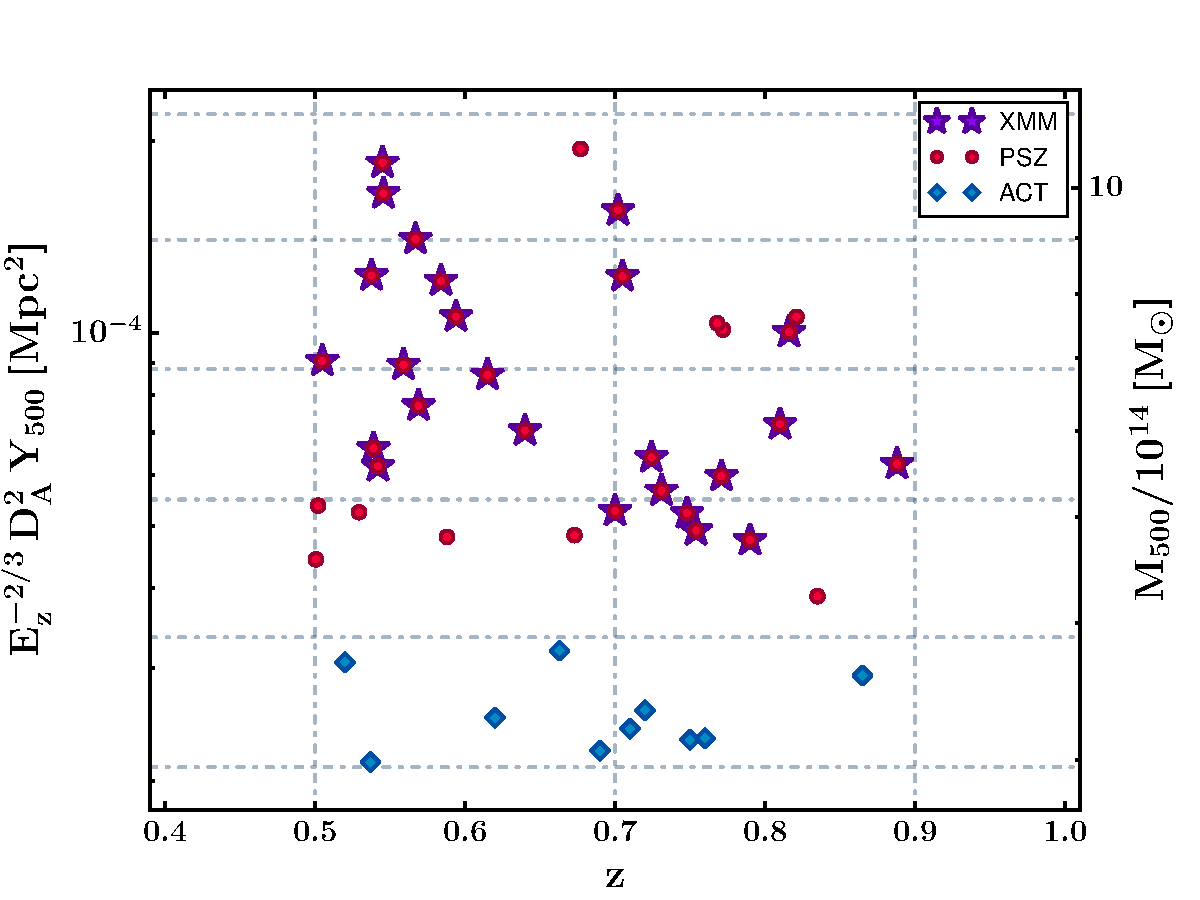
\includegraphics[height=9cm]{LPSZ_M_z_grid.pdf}
\caption{{\footnotesize Galaxy clusters of NIKA2 SZ large program in the mass-redshift plane. The clusters have been selected from the Planck (red dots) and ACT (blue diamonds) catalogs and some clusters are part of the \xmm\ follow-up program (purple stars).}}
\label{fig:LPSZ_grid}
\end{figure*}
\begin{equation}
        y = \frac{\sigma_{\mathrm{T}}}{m_{e} c^2} \int P_{e} \, dl,
        \label{eq:y_compton}
\end{equation}
where $m_{e}$ is the electron rest mass, $\sigma_{\mathrm{T}}$ the Thomson scattering cross section, and $c$ the speed of light. The spherical integral of the ICM pressure distribution enables estimating the integrated Compton parameter $\rm{Y_{tot}}$ that is expected to provide a low-scatter mass proxy for galaxy clusters. In this paper, we consider the spherically integrated Compton parameter up to a cluster radius $\rm{R_{500}}$ for which the mean cluster density is $500$ times the critical density of the Universe.\\
The temperature dependence of the tSZ spectrum is due to relativistic corrections that induce a shift of the null of the tSZ effect and decrease the amplitude of the intensity variation induced by the tSZ effect as the ICM electron temperature increases. We use the results of \cite{ito98,poi98} in the analysis developed in Sect. \ref{subsec:profile_extract} in order to take into account these relativistic corrections when estimating the pressure profile using tSZ maps of galaxy clusters. 

\subsection{The instrument: the NIKA2 camera}\label{subsec:nika2_cam}

The NIKA2 camera is a continuum instrument installed at the 30-m telescope of the Institut de Radioastronomie Millimétrique (IRAM). Three arrays of frequency-multiplexed kinetic inductance detectors \citep[KIDs;][]{mon10,roe12} are installed at the focal plane of the instrument. They enable observing the sky in a field of view of 6.5 arcminutes simultaneously at 150 and 260~GHz. The main beam FWHM measured during the commissioning phase of the camera are respectively 17.7 and 11.2~arcsec at 150 and 260~GHz. The point source sensitivities of the instrument measured in various atmospheric conditions and for different sources are $8~\mathrm{mJy.s^{1/2}}$ and $33~\mathrm{mJy.s^{1/2}}$ at 150 and 260~GHz respectively. Further information on the NIKA2 camera can be found in \cite{ada18}, \cite{cal16}, and \cite{bou16}.\\

The NIKA2 camera is one of the three instruments currently in service that is suitable for high angular resolution tSZ mapping given its resolution, sensitivity and its capacity to observe in two frequency bands. The MUSTANG2 \citep{dic14} camera installed at the \emph{Green Bank Telescope} has a better angular resolution ($9$~arcsec at 90~GHz) but a smaller field of view ($4$~arcmin). The Atacama Large Millimeter/submillimeter Array (ALMA) reaches an angular resolution of $5$~arcsec. However, the tSZ signal can only be mapped in the central part of the observed clusters \citep{kit16}. The NIKA2 camera is therefore a very well suited instrument to map the tSZ signal of high redshift galaxy clusters over a field of view comparable to that of the X-ray observatories used so far to constrain the pressure profile and scaling relation used in cosmological analyses.

\subsection{Sample selection procedure}\label{subsec:sample_select}

The selection strategy considered by the NIKA2 collaboration to build the cluster sample for the NIKA2 SZ large program is mainly motivated by the need to select a representative sample of galaxy clusters. A representative sample is not biased towards a given cluster morphology. It thus makes it possible to characterize the scaling relation $Y_{500}{-}M_{500}$ and the average pressure profile applicable to the entire population of galaxy clusters regardless of their dynamical state. In addition, it can be used to characterize the global properties of clusters and obtain better control of systematic effects generated by astrophysical processes such as fusion with substructures, energy injection into the ICM driven by AGNs or supernovae winds and gas turbulence. Since the integrated Compton parameter is directly related to the thermal energy content within the clusters (see Sect. \ref{subsec:tSZ_effect}), a selection cut on this parameter meets the requirement of establishing a representative sample, unlike a selection based on the X-ray luminosity which favors relaxed clusters with a dense core \citep{ros17}. In order to achieve the scientific goals of the NIKA2 tSZ large programme, the following selection criteria have been considered:

\begin{itemize}
\item The selected clusters must come from catalogs established by observations of the tSZ effect for which information on the cluster redshifts is available.\\
\item The redshift $z$ of the selected clusters must be in the range $0.5 < z < 0.9$ to explore the dynamical and thermodynamic properties of the ICM beyond the local universe.\\
\item The declination of the clusters must be such that $\mathrm{dec} > -11^{\circ}$ to ensure the observability of the selected clusters from the Pico Veleta site where the NIKA2 camera is installed (see Sect. \ref{subsec:nika2_cam}).\\
\end{itemize}

The above criteria have been used in order to select a representative cluster sample from the tSZ catalogs established by the \planck\ and ACT collaborations \citep{pla16b,hil18}. As shown in Figure \ref{fig:LPSZ_grid}, two redshift bins have been considered: $0.5<z<0.7$ and $0.7<z<0.9$. For each redshift range, five mass bins have been defined from selection cuts on the parameter $E_z^{-2/3}\,D_A^2\,Y_{500}$ that is directly related to the mass $M_{500}$ of galaxy clusters. In each of the ten bins thus defined, five galaxy clusters have been selected by maximizing, if possible, the overlap with the \xmm\ follow-up observations of \planck\ clusters. The two bins at low mass contain clusters that could not be detected significantly in the \planck\ survey. The selection of these ten clusters has therefore been made from the ACT catalog (blue diamonds in Fig.  \ref{fig:LPSZ_grid}). The other 35 selected clusters are selected from the \planck\ catalog (red dots in Fig. \ref{fig:LPSZ_grid}) and some are also part of the \xmm\ follow-up program (purple stars in Fig. \ref{fig:LPSZ_grid}). The high redshift bin containing the most massive clusters could not be filled for the moment due to a lack of candidates in the existing tSZ catalogs.

\subsection{Mean pressure profile at high redshift}\label{subsec:goal_szlp}

One of the main goals of the ongoing NIKA2 SZ large program is to explore and test the regularity of the pressure profile of galaxy clusters at $z>0.5$. The applied methodology follows the approach used by \cite{arn10} using the \xmm\ observatory in order to establish the universal pressure profile from a sample of low redshift clusters $z<0.2$ but with an observable, the tSZ effect, that allows to directly probe the pressure distribution in the ICM. In addition, the characterization of the statistical properties of the pressure profile, in relation to the dynamical state of the selected clusters, will bring key information in understanding the selection function of cosmological surveys based on the observation of the tSZ effect as well as the systematic effects affecting analyses based on the study of the tSZ power spectrum. The procedure used in order to constrain the mean pressure profile of the galaxy clusters observed by NIKA2 will be developed in detail in Sect. \ref{subsec:impact_icm_dist}.


\section{The MUSIC simulated sample of galaxy clusters}\label{sec:music_sample}

The fundamental equations of any numerical hydrodynamical simulation are based on a cosmological model as well as on the laws of gravitation and fluid dynamics \citep[See the review of][for more details on N-body simulation techniques.]{dol08}. The main interest of numerical simulations for cosmology comes from their ability to take into account the non-linearities inherent to the large structure formation processes in order to estimate the expected shape of the mass function giving the expected abundance of halos as a function of mass and redshift \citep[\emph{e.g.}][]{tin08}. The mass functions estimated at the end of simulations are therefore assumed to be more realistic than the one obtained from the Press-Schechter theory. This is why they are used in the current cosmological analyses in order to constrain cosmological parameters from cluster surveys.\\

Numerical simulations also enable studying the systematic effects related to known astrophysical processes within galaxy clusters on the characterization of the profiles of their thermodynamic properties and the scaling relations used in cosmological analyses. These studies have become possible because of the constant increase in the number of particles considered in the simulations and therefore in their ability to generate processes for which the characteristic scales are smaller than the typical cluster physical scales. This type of analysis is the main goal of the MUSIC simulation. The purpose of this section is to present the fundamental characteristics of the MUSIC simulation in relation to the analysis developed in this paper. It introduces the basic elements used in Sect. \ref{sec:nika2_simu} as well as the mean thermodynamic properties of the MUSIC clusters that are considered.

\subsection{Overview of the MUSIC simulation}\label{subsec:music_overview}

\begin{figure*}[h!]
\centering
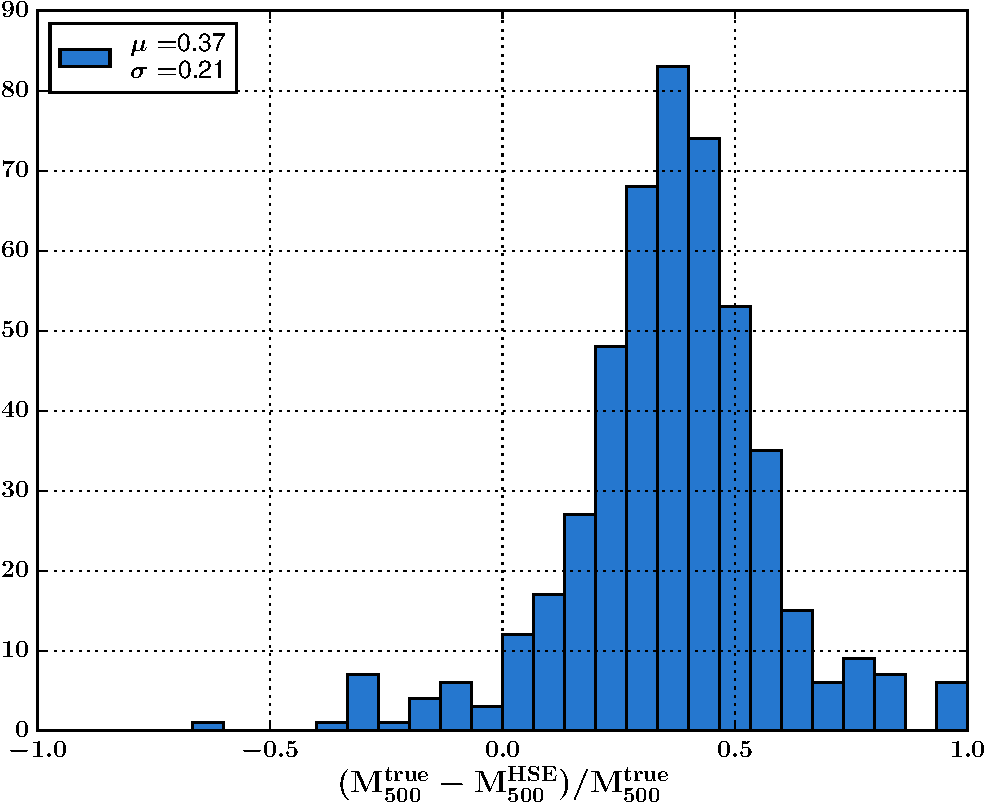
\includegraphics[height=6.6cm]{Histo_mass_MUSIC.pdf}
\hspace{1cm}
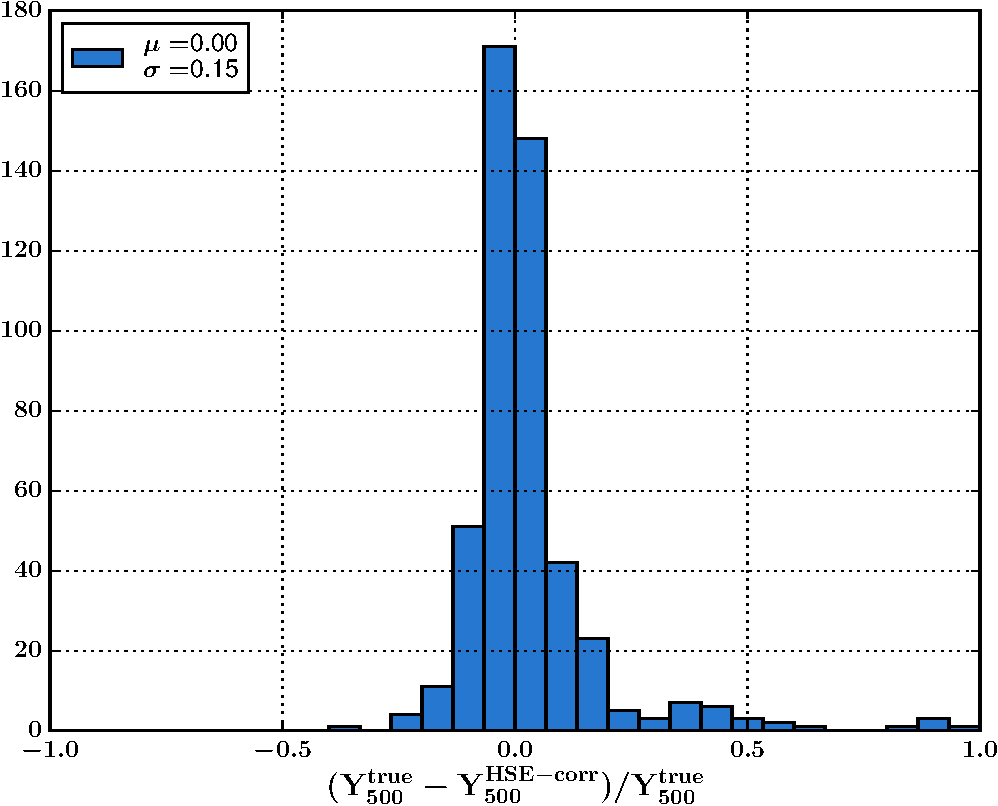
\includegraphics[height=6.6cm]{Histo_Y_MUSIC.pdf}
\caption{{\footnotesize \textbf{Left:} Distribution of the hydrostatic bias values computed for all MUSIC clusters at redshifts $z = 0.54$ and $z = 0.82$. \textbf{Right:} Distribution of the bias on the corrected integrated Compton parameter for the same clusters. The mean and the standard deviation of each histogram are indicated in the upper left corner of the panels.}}
\label{fig:mass_Y500_bias}
\end{figure*}

The MUSIC simulation is based on the cosmological N-body simulation \emph{MultiDark} \citep{pra12}. The latter has been made by considering a cube of $1 \, h^{-1}~\mathrm{Gpc}$ aside. The MUSIC simulation considers the low-resolution execution of \emph{MultiDark} containing a total of $16.8$ million of dark matter particles. The simulation procedure is based on an adaptive mesh refinement grid initialized to a redshift $z=65$. It considers a standard cosmological model according to the parameters constrained by WMAP7, \emph{i.e.} $\Omega_m = 0.27$, $\Omega_b = 0.0469$, $\Omega_{\Lambda} = 0.73$, $h=0.7$, $\sigma_8 = 0.82$, and $n = 0.95$ \citep{kom11}.\\

The 283 most massive halos in the \emph{MultiDark} simulation have been selected in order to be simulated again at high resolution by including gas particles. This new simulation is the MUSIC simulation. The selected systems correspond to clusters with a mass enclosed within the viral radius greater than $10^{15}\, h^{-1}~\mathrm{M_{\odot}}$ at $z=0$ and constitute the MUSIC-2 database considered in the analysis developed in this study. The MUSIC simulation is based on the \emph{GAlaxies with Dark matter and Gas intEracT} (GADGET) code developed by \cite{spr01}. This code is based on the \emph{Smoothed Particle Hydrodynamics} (SPH) numerical method, particularly suitable for describing physical processes related to fluid dynamics such as the ICM. The MUSIC simulation applies the \emph{zoom-in} technique developed by \cite{kly01} that uses the particle phase space trajectories of the \emph{MultiDark} simulation in order to initialize the dynamical quantities of the new particles contained in the 283 selected systems. Each cluster is simulated in a sphere with a radius of $6\, h^{-1}~\mathrm{Mpc}$ at $z=0$ at a resolution such that the masses of dark matter and gas particles are given by $m_{\mathrm{DM}} = 9.0\times 10^8\, h^{-1}~\mathrm{M_{\odot}}$ and $m_{\mathrm{g}} = 1.9\times 10^8\, h^{-1}~\mathrm{M_{\odot}}$ respectively. The regions adjacent to each sphere are also simulated with a decreasing resolution with radius until the resolution of the \emph{MultiDark} simulation is reached. This enables taking into account the physical processes located in the periphery of the MUSIC clusters while optimizing the computing time allocated to the simulation. In addition to the standard equations of gravitation and fluid dynamics, the MUSIC simulation includes additional physical processes such as gas cooling by thermal emission, stellar formation and energy injection into the environment by supernovae winds \citep{spr03}. A total of fifteen instant captures of the properties of each cluster are made between the initial redshift $z=9$ considered by MUSIC and $z=0$. These captures enable tracing the dynamical behavior of the MUSIC clusters over the relevant redshift interval to study the galaxy cluster formation processes.\\

The analysis developed in this paper relies on the MUSIC snapshots made at redshifts $z=0.54$ and $z=0.82$ in order to study the thermodynamic properties of the MUSIC clusters in a range of redshifts that is similar to the one considered for NIKA2 SZ large program. The MUSIC clusters at redshifts $z=0.54$ and $z=0.82$ are thus said to be members of bins 1 and 2 respectively.

\subsection{MUSIC \emph{y}-maps and 3D pressure profiles}\label{subsec:music_products}

\begin{figure*}[h!]
\centering
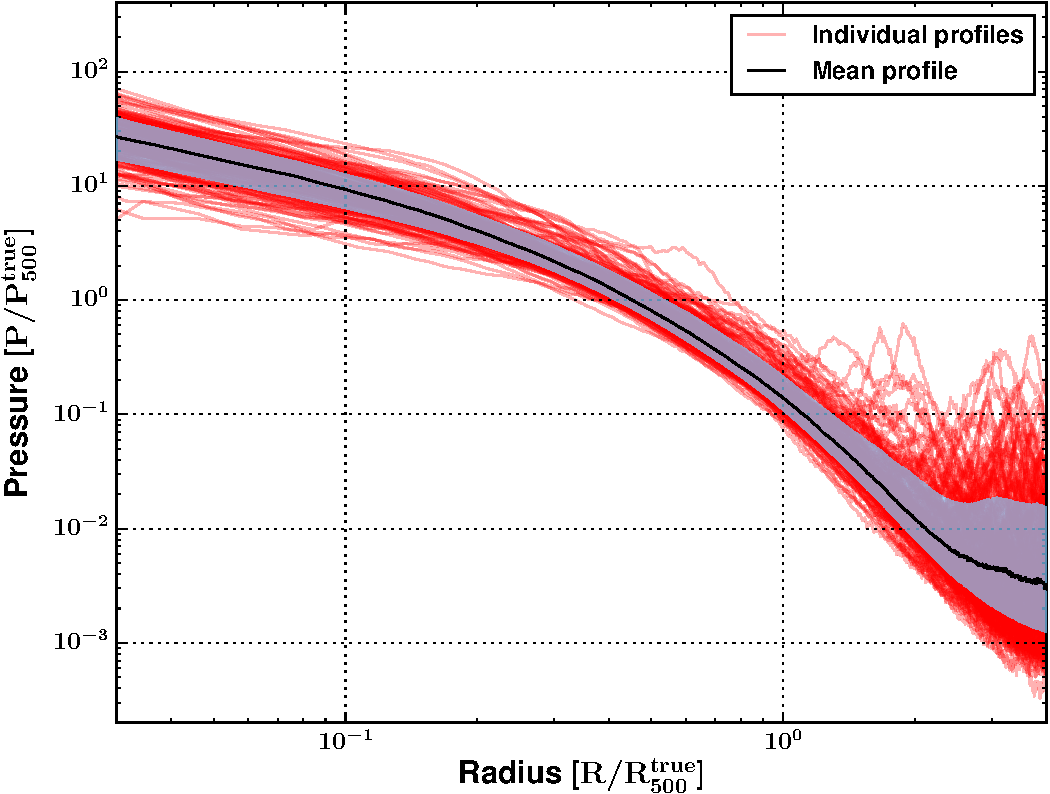
\includegraphics[height=6.6cm]{MUSIC_individuals_bin1.pdf}
\hspace{0.6cm}
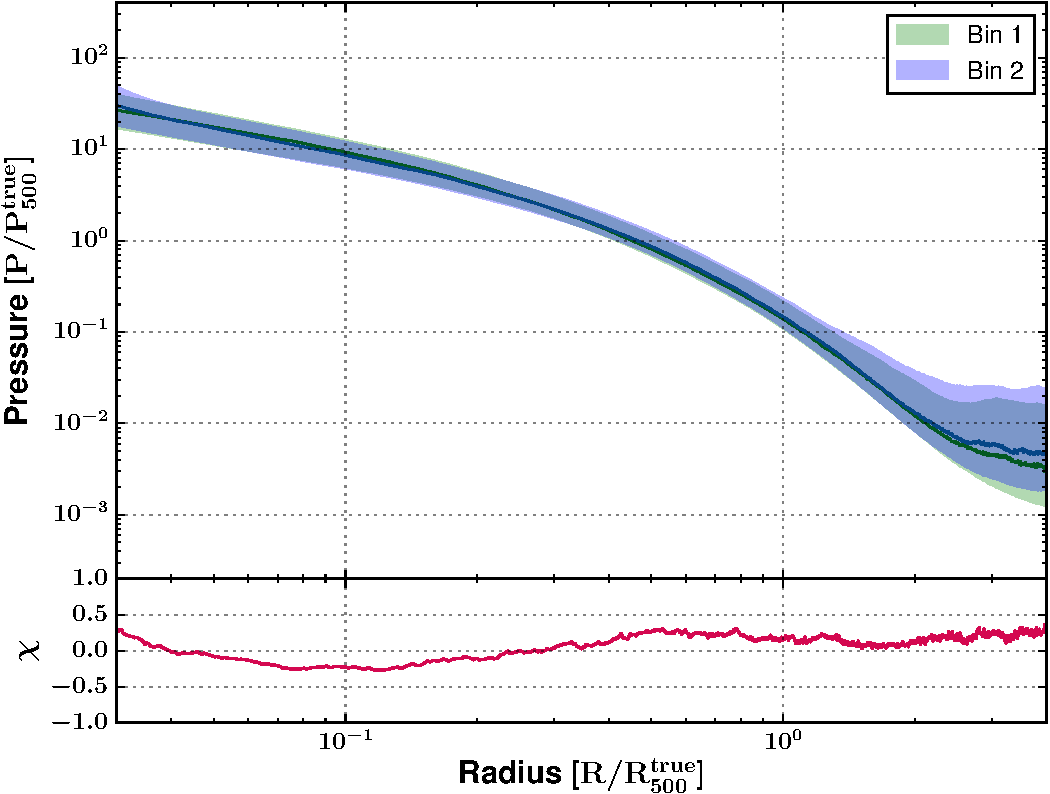
\includegraphics[height=6.6cm]{MUSIC_compare_bin1_bin2.pdf}
\caption{{\footnotesize \textbf{Left:} Normalized pressure profiles extracted from the MUSIC simulation for all the clusters located at a redshift $z=0.54$ (red lines). The mean pressure profile is represented in black and the intrinsic scatter of the distribution at $1\sigma$ is given by the blue region. \textbf{Right:} Comparison of the mean normalized pressure profiles estimated from the MUSIC profiles extracted at $z=0.54$ (green), and at $z=0.82$ (blue). The difference between the two profiles weighted by the mean of their associated uncertainties is shown in red in the lower panel.}}
\label{fig:MUSIC_P_profiles}
\end{figure*}

In order to carry out an analysis of the impact of the ICM disturbances that can be identified by NIKA2 on the estimation of the pressure profile at high redshift, it is necessary to obtain Compton parameter maps and thermodynamic profiles associated with each simulated cluster.\\

Compton parameter maps are computed by considering a single line of sight for each cluster. The pressure associated with the gas particles contained in a cylinder is integrated along its rotation axis, aligned with the considered line of sight. The length of the cylinder corresponds to six times the virial radius $R_{\mathrm{vir}}$ of the considered cluster and its base has a radius equal to $3R_{\mathrm{vir}} \simeq 5R_{500}$. The MUSIC Compton parameter maps are all defined on a square grid of 10~Mpc on each side with a pixel size of 10~kpc. At the redshifts considered for this study, this corresponds to a field of view of about 23~arcmin large and a pixel resolution of about 1.4~arcsec. These maps are therefore perfectly adapted to the instrumental characteristics of NIKA2 because the spatial distribution of the tSZ signal is defined over the entire NIKA2 field of view and the pixel size is small enough compared to the beam extension of NIKA2 at 150~GHz. The MUSIC Compton parameter maps are used in the method developed in Sect. \ref{sec:nika2_simu} to simulate the NIKA2 and \planck\ tSZ maps of the selected MUSIC clusters.\\

It is also necessary to obtain the thermodynamic profiles of the MUSIC clusters in order to constrain the impact of ICM disturbances on the pressure profile estimated by deprojection of the tSZ signal from the simulated maps. The radial distributions of the ICM pressure, density, temperature, entropy and the cluster total mass are calculated for each cluster at the two redshifts considered by averaging the values of the thermodynamic quantities associated with the particles of the simulation in concentric spherical shells. The total sphere considered has a radius equal to $3R_{\mathrm{vir}}$ and the thickness of the spherical shells is 10~kpc. The uncertainty associated with each pressure point corresponds to the error on the mean of the pressure values contained in the considered spherical shells. The uncertainties on the profiles increase in the cluster outskirts due to the increase in the standard deviation of the thermodynamic quantities caused by deviations from spherical symmetry and hydrostatic equilibrium in these regions. Moreover, it should be noted that the decrease in the resolution of the simulation in the periphery of the clusters (see Sect. \ref{subsec:music_overview}), implies that the number of particles considered to average the thermodynamic quantities is also reduced. The pressure profiles extracted directly from the simulation are nevertheless perfectly constrained from the center of the clusters to radii in the order of $3R_{500}$. They will thus be compared in Sect. \ref{subsec:impact_icm_dist} to the pressure distribution estimated by deprojection of the tSZ signal in the simulated NIKA2 maps.

\subsection{Integrated parameters of the MUSIC synthetic clusters}\label{subsec:music_integ}

In order to determine the intrinsic dynamical properties of the MUSIC clusters, we estimate the mass and integrated Compton parameter of each cluster at the two considered redshifts. The quantities $M_{500}$ and $Y_{500}$ represent the fundamental quantities for cosmological analyses. The mass $M_{500}$ is defined from the radius $R_{500}$ using the following relation:
\begin{equation}
M_{500} = \frac{4}{3}\pi R_{500}^3 \times 500\rho_c
\label{eq:M500MUSIC}
\end{equation}
The integrated Compton parameter $Y_{500}$ is obtained by the spherical integral of the pressure profile up to $R_{500}$. The $R_{500}$ radius is therefore an essential quantity to define the integrated parameters of the clusters. The mass profile $\mathrm{M}(r)$ of each simulated cluster is used to calculate a mean matter density profile $\langle \rho \rangle (r)$ using the volume profile $V(r) = \frac{4}{3}\pi r^3$ to define the radius $R_{500}$ and therefore the quantities $M_{500}$ and $Y_{500}$. We use two different procedures to estimate the mass profile $\mathrm{M}(r)$ considered to define the radius $R_{500}$ of the simulated clusters.\\
The first is based on the total mass profile $\mathrm{M^{true}}(r)$ extracted from the MUSIC simulation by averaging the mass induced by dark matter and gas particles inside spherical shells. The radius $R_{500}^{\mathrm{true}}$ is estimated from the mean matter density profile obtained through this mass profile. The equation (\ref{eq:M500MUSIC}) is used to calculate $M_{500}^{\mathrm{true}}$. The pressure profile extracted from the simulation (see Sect. \ref{subsec:music_products}) is integrated up to $R_{500}^{\mathrm{true}}$ to estimate $Y_{500}^{\mathrm{true}}$.\\

\begin{figure*}[h!]
\centering
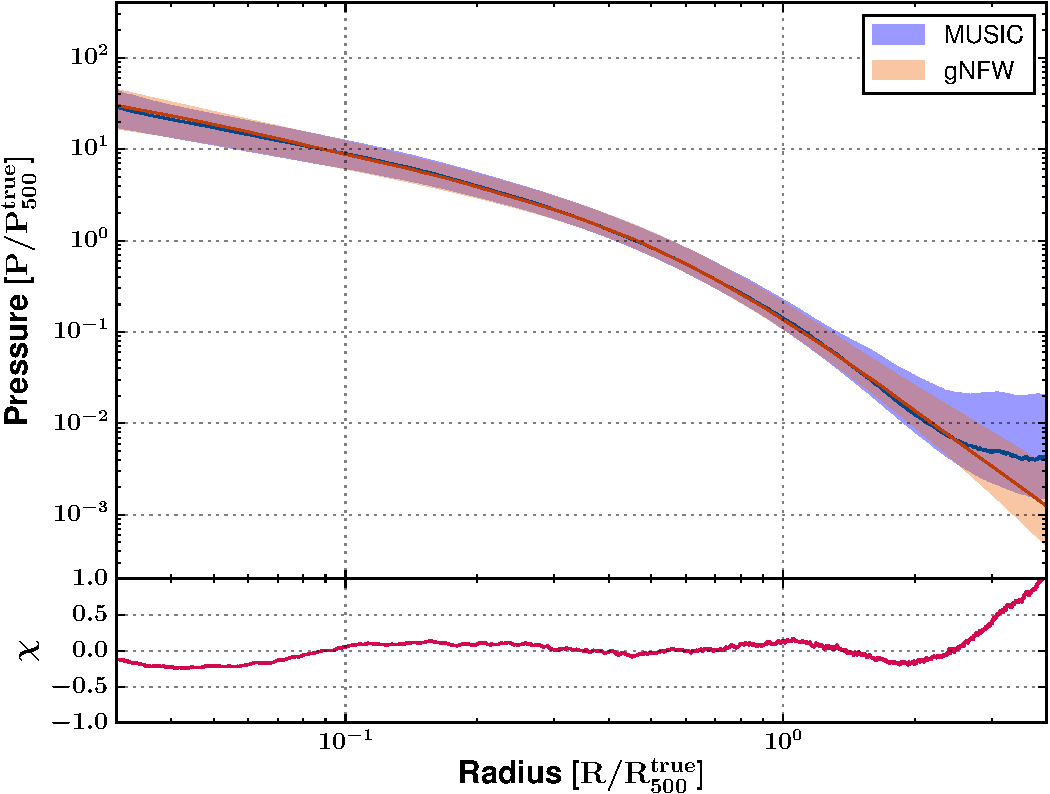
\includegraphics[height=6.6cm]{MUSIC_compare_with_gNFW.pdf}
\hspace{0.6cm}
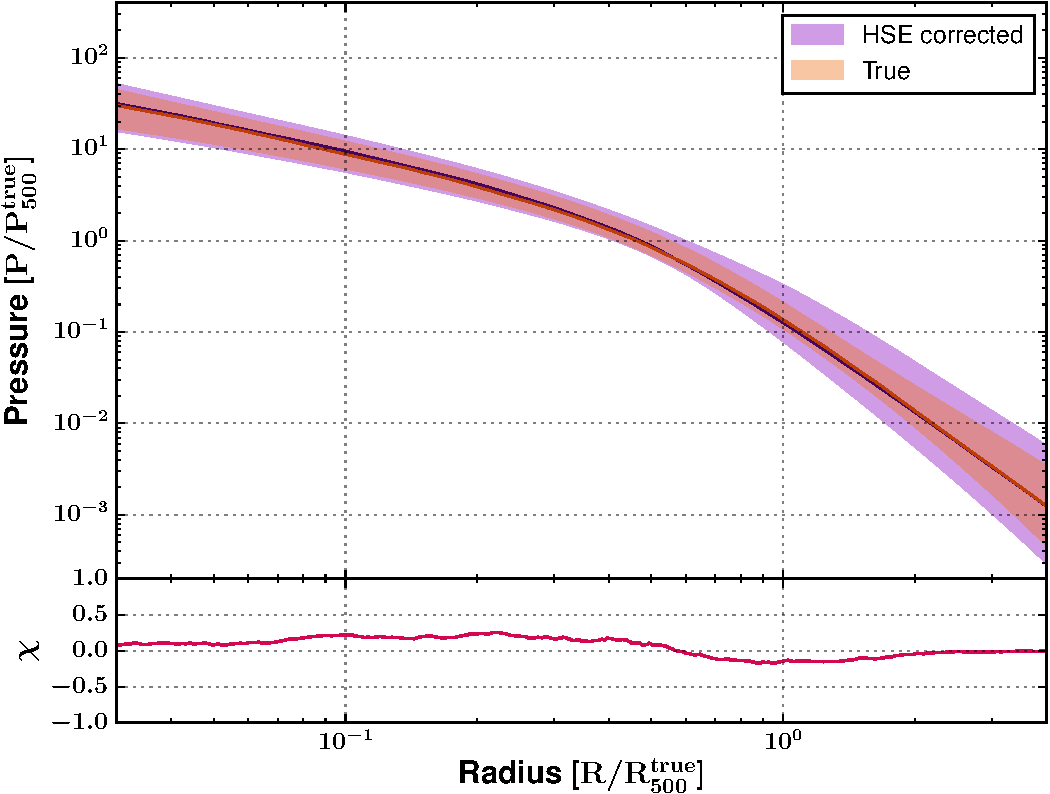
\includegraphics[height=6.6cm]{MUSIC_compare_HSE_corr.pdf}
\caption{{\footnotesize \textbf{Left:} Mean normalized pressure profiles estimated by considering the profiles extracted from the MUSIC simulation (blue) and the gNFW fits of these profiles (orange) for each cluster at $z=0.54$ and $z=0.82$. \textbf{Right:} Mean pressure profiles obtained by normalizing the gNFW profiles associated with each MUSIC cluster by the values of $R_{500}^{\mathrm{true}}$ and $P_{500}^{\mathrm{true}}$ (orange) and by the values of $R_{500}^{\mathrm{HSE-corr}}$ and $P_{500}^{\mathrm{HSE-corr}}$ obtained after correction of the hydrostatic mass of each cluster by the mean hydrostatic bias of the MUSIC simulation at the two considered redshifts (magenta). The differences between the two profiles weighted by the mean of their associated uncertainties are shown in red in each lower panel.}}
\label{fig:MUSIC_gNFW_HSE}
\end{figure*}

The second is related to the fact that the observations made by NIKA2 for its SZ large program cannot be used to estimate the radius $R_{500}^{\mathrm{true}}$ because the mass profile can only be calculated under the assumption of hydrostatic equilibrium by considering the estimated pressure profile and a gas density profile deprojected from X-ray observations. We thus calculate for each MUSIC synthetic cluster the hydrostatic mass profile $\mathrm{M^{HSE}}(r)$ by combining their pressure $P_e(r)$ and density $n_e(r)$ profiles using the following equation:
\begin{equation}
\mathrm{M^{HSE}}(r) = -\frac{r^2}{G\mu m_p n_e(r)} \times \frac{d \, P_e(r)}{dr}
\label{eq:mass_HSE}
\end{equation}
where $m_p$ is the proton mass, $\mu$ is the mean molecular weight\footnote{Mass of the ICM particles in proton mass units ($m = \mu m_p$)}, and $G$ is the gravitational constant. This profile is used in the same way as the mass profile $\mathrm{M^{true}}(r)$ in order to estimate the value of $R_{500}^{\mathrm{HSE}}$. The latter allows us to define the integrated quantities $M_{500}^{\mathrm{HSE}}$ and $Y_{500}^{\mathrm{HSE}}$ associated with each MUSIC cluster.\\

The estimates of the true total mass of the simulated clusters and their mass calculated under the hydrostatic equilibrium hypothesis make it possible to constrain the value of the hydrostatic bias for each MUSIC cluster:
\begin{equation}
b = \frac{M_{500}^{\mathrm{true}} - M_{500}^{\mathrm{HSE}}}{M_{500}^{\mathrm{true}}}
\end{equation}
The mean of the $b$ values obtained at the two considered redshifts are perfectly compatible\footnote{We observe a relative difference of 4\% between the mean hydrostatic biases estimated at the two redshifts.}. The left panel of Fig. \ref{fig:mass_Y500_bias} represents the distribution of the $b$ values for all the MUSIC clusters at $z=0.54$ and $z=0.82$. The mean hydrostatic bias associated with the MUSIC clusters is given by $\mu_b = 0.37$ which is compatible with the observations made by the project \emph{Weighing the Giants} \citep{lin14} although higher than most current constraints between 0.1 and 0.3 \citep[see \emph{e.g.} Fig. 10 in][]{sal18}. We also observe on the histogram of the $b$ values obtained in the simulation that the hydrostatic bias is subject to a large scatter: $\sigma_b = 0.21$.\\ 

The hydrostatic bias associated with each cluster of the NIKA2 SZ large program is not known \emph{a priori}. The hydrostatic mass $M_{500}^{\mathrm{HSE}}$ is thus usually corrected using the mean hydrostatic bias from the results of other studies. In the case studied here, we estimate the corrected hydrostatic mass of each MUSIC cluster using the following relation:
\begin{equation}
M_{500}^{\mathrm{HSE-corr}} = M_{500}^{\mathrm{HSE}} / (1 - \mu_b)
\end{equation}
The correction of the hydrostatic mass measured by the mean hydrostatic bias makes it possible to cancel on average the bias observed between the mass estimates but has no effect on the dispersion $\sigma_b$ of the distribution. Using the mass $M_{500}^{\mathrm{HSE-corr}}$ allows us to define a value of $R_{500}^{\mathrm{HSE-corr}}$ by applying the equation (\ref{eq:M500MUSIC}) that can be used to estimate the integrated Compton parameter $Y_{500}^{\mathrm{HSE-corr}}$ for each cluster. The right panel of Fig. \ref{fig:mass_Y500_bias} shows the histogram of the bias on the $Y_{500}$ measurement made by considering the estimate of the $R_{500}^{\mathrm{HSE-corr}}$ radius as an outer boundary of the integral of the pressure profile of each cluster instead of the $R_{500}^{\mathrm{true}}$ radius. The histogram obtained is centered on 0 but has a standard deviation of 15\%. The use of the hydrostatic equilibrium hypothesis and a mean hydrostatic bias thus induces an additional scatter over all the measured integrated quantities. The $Y_{500}{-}M_{500}$scaling relation calibrated using X-ray and tSZ measurements therefore has an increased dispersion compared to its intrinsic dispersion due to the use of the hydrostatic equilibrium hypothesis. It will be important to take this systematic effect into account when the tSZ-mass scaling relation associated with the sample of the NIKA2 SZ large program will be estimated.

\subsection{Mean pressure profile of the MUSIC synthetic clusters}\label{subsec:music_prof}

\begin{figure*}[h!]
\centering
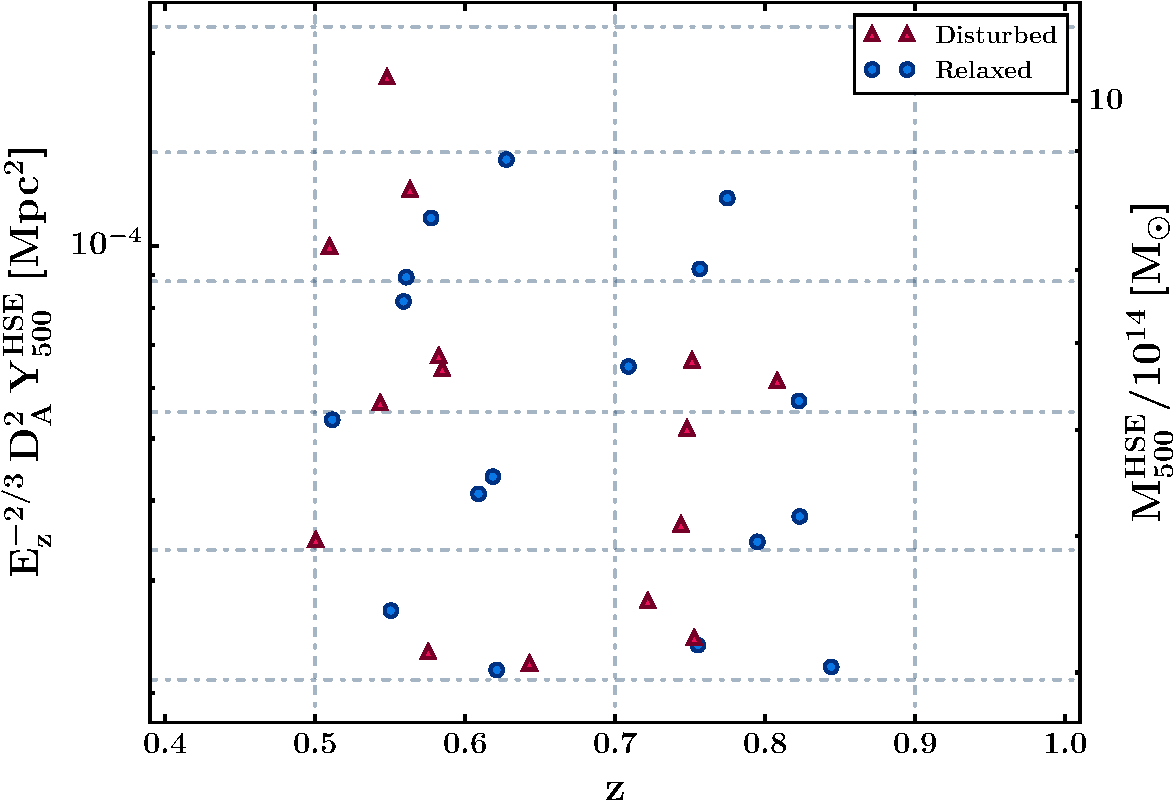
\includegraphics[height=9cm]{Simulated_NIKA2_sample.pdf}
\caption{{\footnotesize Distribution of the selected MUSIC clusters in the mass-redshift plane. The mass and redshift bins considered are identical to those of NIKA2 SZ large program (see Fig. \ref{fig:LPSZ_grid}). Morphologically relaxed and disturbed clusters are indicated by blue dots and red triangles respectively.}}
\label{fig:MUSIC_NIKA2_sample}
\end{figure*}

The objective of this paper is to study the NIKA2 ability to constrain the impact of ICM disturbances on the mean pressure profile and its associated scatter at high redshift. The uncertainty associated with the mean pressure profile also takes into account the number of profiles considered for its estimation and can be propagated in a cosmological analysis based on a tSZ survey up to the constraints on the cosmological parameters. However, we will be more interested in the intrinsic scatter associated with the mean pressure profile of a cluster sample in this study as it corresponds to the potential systematic error made in the case where the self-similarity hypothesis cannot be applied to the whole cluster population.\\

We estimate the mean pressure profiles of the MUSIC clusters by considering all their associated profiles at $z=0.54$ and $z=0.82$. The left panel of Fig. \ref{fig:MUSIC_P_profiles} represents all the pressure profiles (red curves) of the MUSIC synthetic clusters at redshift $z=0.54$ after normalization of the radius by the value of $R_{500}^{\mathrm{true}}$ associated with each cluster and the pressure by the amplitude factor $P_{500}^{\mathrm{true}}$ giving the scaling relation between the pressure content and the cluster total mass in the self-similar model:
\begin{equation}
P_{500}^{\mathrm{true}} = 1.65 \times 10^{-3} \, h(z)^{8/3} \, \left[ \frac{M_{500}^{\mathrm{true}}}{3 \times 10^{14} \, h_{70}^{-1}~\mathrm{M_{\odot}}}\right]^{2/3} \, h_{70}^2~\mathrm{keV} \, \mathrm{cm^{-3}}
\end{equation}
where $h(z)$ is the ratio of the Hubble constant at redshift $z$ to its present value $H_0$, and $h_{70} = H_0 / 70$. The normalized pressure distribution is modelled at each radius by an asymmetric log-normal distribution\footnote{The logarithm of the pressure is modeled by a Gaussian with two distinct standard deviations on either side of the distribution peak.} in order to constrain the mean pressure profile and its intrinsic dispersion. The computed profile is represented by a black line on the left panel of Fig. \ref{fig:MUSIC_P_profiles} and the standard deviation at $1\sigma$ of the distribution of the normalized pressure profiles is given by the blue region. The mean pressure profile shows a flattening for radii $r>2R_{500}$. In addition, the dispersion of the profile distribution increases significantly in the same radius range. This is due to the deviations from the gas dynamic equilibrium at radii larger than the virial radius. Accretion of the surrounding environment and the presence of dense substructures and gas shocks in these regions lead to an increase in the mean thermal pressure and fluctuations of the latter, respectively responsible for the flattening of the mean pressure profile and the increase of its associated scatter.\\

An identical analysis is performed for the pressure profiles associated with the MUSIC clusters at redshift $z=0.82$. The mean pressure profiles obtained at the two redshifts considered are represented in blue and green on the right panel of Fig. \ref{fig:MUSIC_P_profiles}. The red curve shown on the lower panel of the figure corresponds to the difference between the two profiles weighted by the mean dispersion observed at each radius. We note that no significant variation in the shape and amplitude of the mean pressure profile is observed between the redshifts $z=0.54$ and $z=0.82$ of the MUSIC simulation. We therefore choose to consider a mean pressure profile combining all the profiles estimated in bins 1 and 2 in the analysis developed in Sect. \ref{subsec:impact_icm_dist}.\\

In order to reduce the analysis time associated with the estimation of the pressure profile of each cluster considered in the study developed in Sect. \ref{subsec:profile_extract}, we choose to model the pressure distribution in the ICM by a parametric generalized Navarro-Frenk-White profile \citep[gNFW, ][]{nag07},
\begin{equation}
        P_e(r) = \frac{P_0}{\left(\frac{r}{r_p}\right)^c \left(1+\left(\frac{r}{r_p}\right)^a\right)^{\frac{b-c}{a}}},
\label{eq:gNFW}
\end{equation}
where $P_0$ is a normalization constant, $r_p$ is a characteristic radius, and $a$ characterizes the size of the transition between the two profile slopes $b$ and $c$ at large and small radii respectively. This model is therefore defined by only five free parameters while a non-parametric profile contains more than twice as many for typical observations with NIKA2 \citep{rup18}. It is therefore necessary to check whether the gNFW model is appropriate to describe the mean pressure profile of the MUSIC clusters at the considered redshifts. Each pressure profile extracted from the MUSIC simulation at both redshifts is therefore fitted by a gNFW model and normalized by the corresponding values of $R_{500}^{\mathrm{true}}$ and $P_{500}^{\mathrm{true}}$. The resulting distribution of gNFW profiles is used to estimate the mean pressure profile and its associated scatter. The estimated profile is represented by the orange line on the left panel of Fig. \ref{fig:MUSIC_gNFW_HSE}. The mean pressure profile estimated using the gNFW model is compared to the mean profile obtained by considering the pressure profiles extracted directly from the simulation (blue line). The weighted difference between the profiles is shown in the lower panel (red line). We do not observe any significant discrepancy between the two profiles for radii $r<3R_{500}$. In addition, the difference caused by the flattening of the pressure profiles extracted from the simulation observed between the mean profiles for radii greater than $3R_{500}$, results in a relative difference on the integrated Compton parameter $Y_{\mathrm{5R500}}$ of about 6\%. This difference is four times smaller than the typical relative uncertainty on the integrated tSZ flux measured by \planck\ \citep{pla16b}. The gNFW profile is therefore perfectly adapted to model the pressure distribution of the MUSIC clusters from a combined NIKA2/\planck\ analysis (see Sect. \ref{subsec:profile_extract}).\\


\begin{figure*}[h!]
\centering
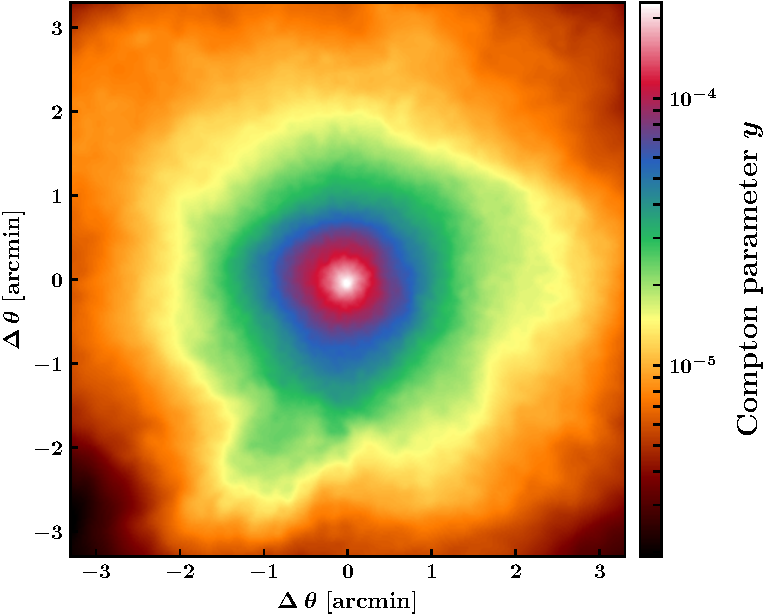
\includegraphics[height=6.6cm]{Definition_relax.pdf}
\hspace{0.6cm}
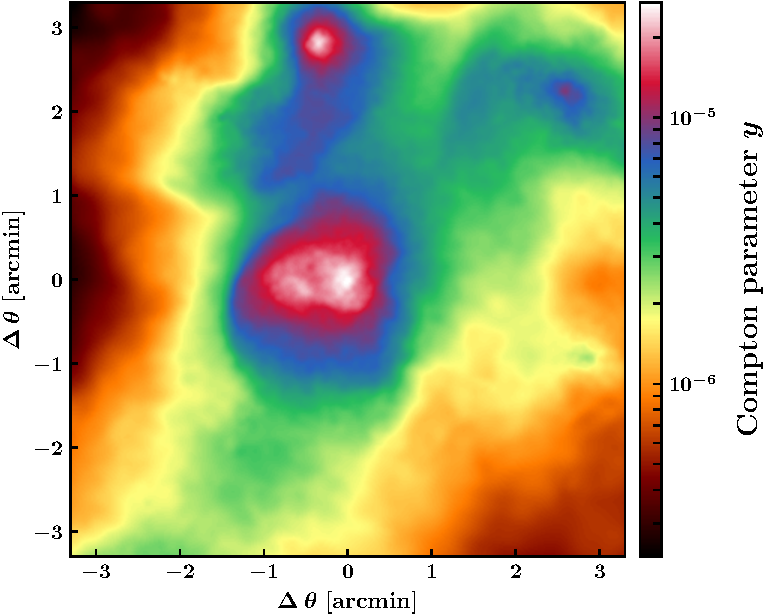
\includegraphics[height=6.6cm]{Definition_disturbed.pdf}
\caption{{\footnotesize \textbf{Left:} MUSIC Compton parameter map of a cluster considered as a relaxed system in the definition of the simulated cluster sample in Sect. \ref{subsec:simu_obs}.  \textbf{Right:} MUSIC Compton parameter map of a cluster considered as a disturbed system. This represents an extreme case where both individual substructures and an extension of the ICM of the main halo are clearly identified.}}
\label{fig:def_relax_disturbed}
\end{figure*}

Using the hydrostatic equilibrium hypothesis also has an effect on the mean pressure profile estimated from tSZ observations. As shown in Sect. \ref{subsec:music_integ} the value of $R_{500}^{\mathrm{HSE-corr}}$ estimated from the total mass, under the assumption of hydrostatic equilibrium, corrected by the mean hydrostatic bias, is not biased but is scattered around the value of $R_{500}^{\mathrm{true}}$. The same conclusion is made if we consider the normalization coefficient $P_{500}^{\mathrm{HSE-corr}}$. As shown on the right panel of Fig. \ref{fig:MUSIC_gNFW_HSE}, the mean pressure profile obtained under the hydrostatic equilibrium assumption by correcting the integrated quantities by the mean hydrostatic bias (magenta curve) is identical to the mean pressure profile obtained by considering the true values of $R_{500}$ and $P_{500}$ for the normalization (orange curve). However, its associated scatter is 5 to 60\% higher for radii greater than $0.5R_{500}$. The estimation of the intrinsic scatter of the distribution of pressure profiles at high redshift is important for cosmological analyses as it traces the potential systematic uncertainty associated with the cluster self-similarity assumption. It is therefore important to investigate whether this increase in dispersion associated with the mean pressure profile, caused by the use of the hydrostatic equilibrium hypothesis, is comparable to the additional dispersion induced by systematic effects due to disturbances of the ICM on the reconstruction of the pressure profile from NIKA2 tSZ observations. Understanding the origin of the different processes responsible for the dispersion of pressure profiles estimated from tSZ observations will eventually allow us to establish methods that take these systematic effects into account in cosmological analyses.

\section{Simulation of the NIKA2 SZ large program observations}\label{sec:nika2_simu}

The goal of this section is to present the method used in order to simulate NIKA2 and \planck\ tSZ maps of a sample of MUSIC clusters similar to the one considered for the NIKA2 SZ large program. These maps constitute the data set used in the analysis developed in Sect. \ref{sec:mean_prof} to study the effect of ICM perturbations on the estimation of the mean pressure profile using the NIKA2 tSZ analysis pipeline.

\subsection{Definition of the NIKA2 cluster sample}\label{subsec:nika2_sample}

The galaxy cluster selection procedure used for the NIKA2 SZ large programme (see Sect. \ref{subsec:sample_select}) is applied to establish a simulated cluster sample based on the MUSIC data. In order to reduce the analysis time required in the study developed in Sect. \ref{subsec:profile_extract} without increasing significantly the statistical uncertainties on the estimation of the mean pressure profile, we choose to populate each mass and redshift bin considered for the NIKA2 SZ large program by four MUSIC clusters instead of five. The number of clusters selected is thus comparable to the one considered for the NIKA2 SZ large program. The distribution of the clusters selected to simulate the NIKA2 SZ large program in the mass-redshift plane is shown in Fig. \ref{fig:MUSIC_NIKA2_sample}. The redshifts associated with each cluster are generated randomly using a uniform distribution within their respective bins for display reasons. All the simulated clusters of bin 1 are actually located at a redshift $z=0.54$ and those of bin 2 at a redshift $z=0.82$. Since the cluster selection procedure of the NIKA2 SZ large program has been carried out by applying a mass cut in the \planck\ and ACT catalogs (see Sect. \ref{subsec:sample_select}), the hydrostatic mass estimates of the MUSIC clusters $M_{500}^{\mathrm{HSE}}$ are used in order to select the MUSIC clusters from the whole simulated sample. We only consider MUSIC clusters with a mass greater than $3\times 10^{14}~\mathrm{M_{\odot}}$ in order to populate the considered mass and redshift bins. This cut reduces the size of the initial MUSIC sample to a total of 82 clusters at $z=0.54$ and 42 clusters at $z=0.82$. Because the mass function decreases as a power law with both the mass and the redshift of galaxy clusters, the limited volume of the \emph{MultiDark} simulation cube that enabled simulating the global properties of the MUSIC clusters is not large enough to populate the highest mass bin of the high redshift bin (see Fig. \ref{fig:MUSIC_NIKA2_sample}). In addition, the highest mass bin of the first redshift bin and the second-last mass bin of the high redshift one cannot be completely filled for the same reason. Since the fraction of clusters with a disturbed ICM at high redshift is an unknown parameter, we choose to establish a sample containing an equivalent number of dynamically relaxed and disturbed clusters. The other mass and redshift bins are thus populated by choosing two morphologically relaxed and two disturbed clusters among all the MUSIC clusters available in each bin.\\

\begin{figure*}[h!]
\centering
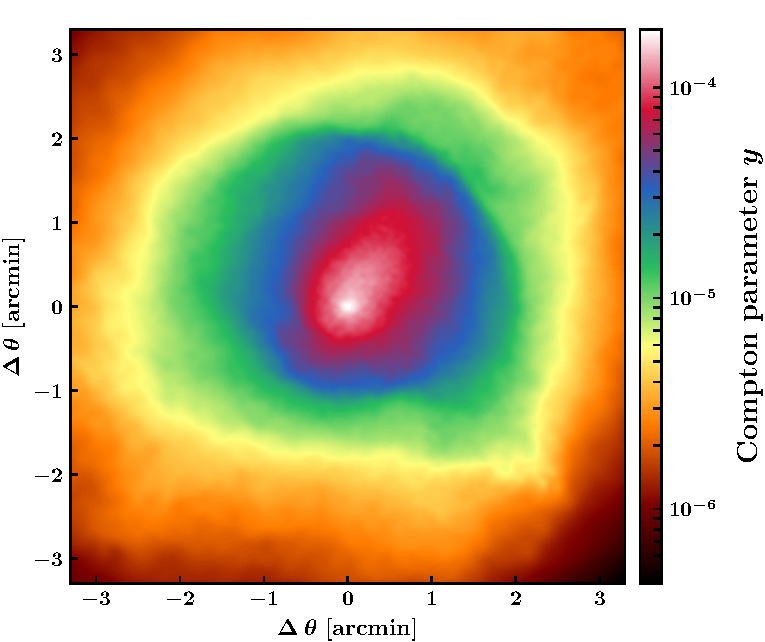
\includegraphics[height=4.8cm]{Simu_NK2_Pla_maps1.pdf}
\hspace{0.3cm}
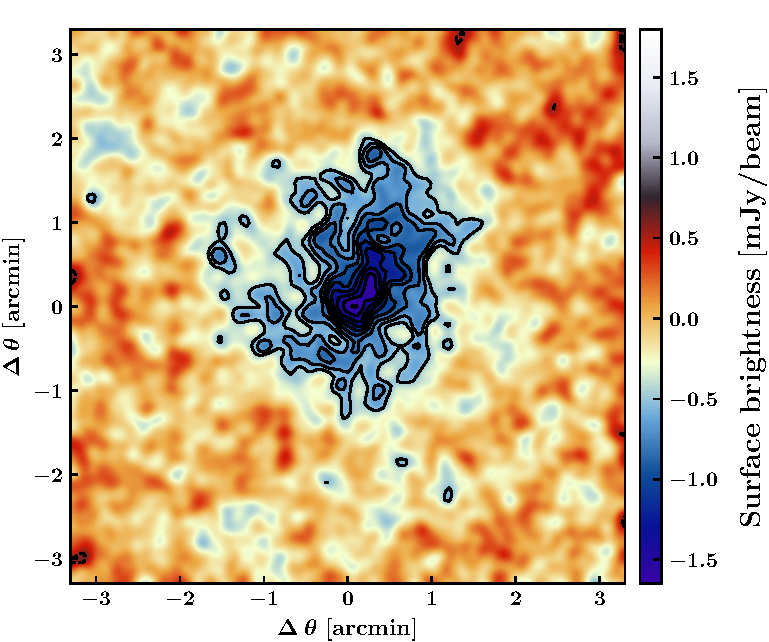
\includegraphics[height=4.8cm]{Simu_NK2_Pla_maps2.pdf}
\hspace{0.3cm}
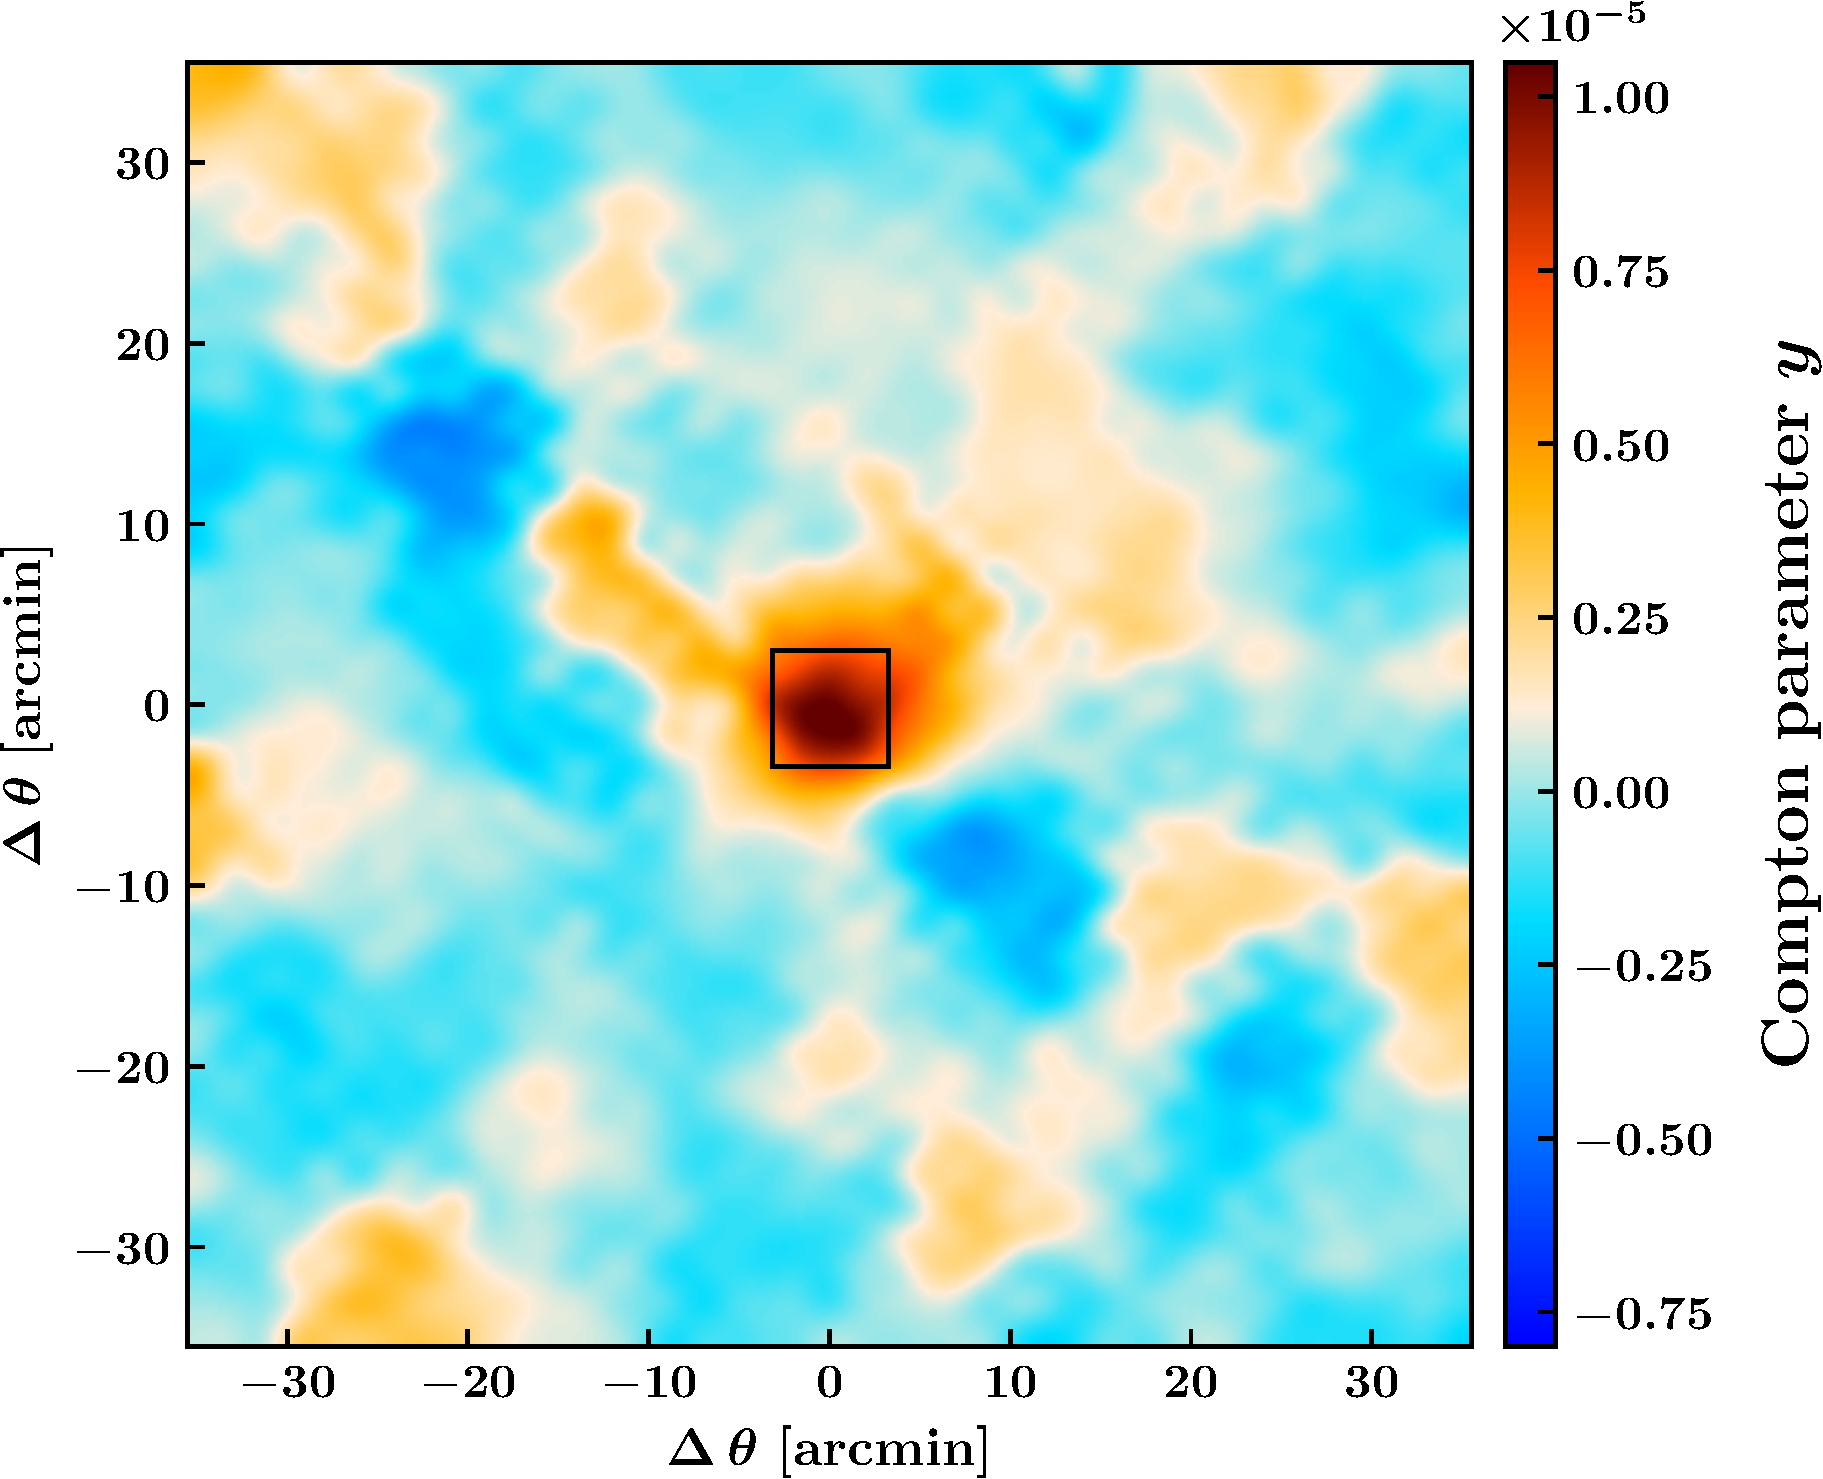
\includegraphics[height=4.8cm]{Simu_NK2_Pla_maps3.pdf}
\caption{{\footnotesize \textbf{Left:} MUSIC Compton parameter map of a selected disturbed cluster in the first redshift bin. An ICM extension is clearly identified in the top-right region of the map.  \textbf{Middle:} Simulated NIKA2 tSZ surface brightness map at 150~GHz of the MUSIC cluster shown in the left panel. \textbf{Right:} Simulated \planck\ Compton parameter map of the MUSIC cluster shown in the left panel. The field of view considered for the left and middle panels is shown as a black rectangle at the center of the map.}}
\label{fig:simu_nk2_pla_maps}
\end{figure*}

Estimating the dynamical state of the MUSIC clusters by morphological considerations is first performed by a visual inspection of the Compton parameter maps of the MUSIC clusters in each bin. As shown on the left panel of Fig. \ref{fig:def_relax_disturbed}, a cluster is considered morphologically relaxed if it has a single tSZ surface brightness peak and its two-dimensional structure has a symmetry close to circular symmetry\footnote{this does not exclude triaxial clusters whose major axis is aligned with the line of sight}. On the other hand, the so-called disturbed clusters (see right panel of Fig. \ref{fig:def_relax_disturbed}) have a number of tSZ peaks greater than or equal to two or an obvious deviation from the circular symmetry. The $M$ morphological indicator introduced by \cite{cia18} to discriminate dynamically relaxed and disturbed clusters from Compton parameter maps is also used to confirm the selection made by visual inspection. This indicator combines several estimators of the dynamical state of the clusters such as the offset between the position of the tSZ peak and the tSZ surface brightness barycenter or the ratio between the tSZ flux integrated in the core region of the cluster and the one integrated up to the viral radius. After analyzing the properties of the $M$ indicator, Cialone \emph{et al.} have concluded that dynamically relaxed clusters are such that $M<-0.41$ and disturbed clusters verify $M>0.41$. The intermediate $M$ values form a mixed class where the dynamical state of the clusters is not clearly defined. The relaxed clusters in bin 1 have an average morphological indicator $M = -0.74 \pm 0.12$ and are indicated by blue dots in Fig. \ref{fig:MUSIC_NIKA2_sample} and disturbed clusters (red triangles) of the same redshift bin are such that $M = 0.52 \pm 0.18$. The clusters of the second redshift bin verify $M = -0.61 \pm 0.11$ for relaxed clusters and $M = 0.82\pm 0.31$ for disturbed clusters. We thus note an agreement between the visual characterization of the morphology of the selected clusters with the results given by the $M$ indicator. The defined cluster sample therefore has a fraction of relaxed clusters of about 50\%. This sample of MUSIC clusters is then processed as the sample of clusters from the NIKA2 SZ large program would be in order to constrain the mean ICM pressure profile.

\subsection{Simulation of NIKA2 and \planck\ SZ observations}\label{subsec:simu_obs}

This section describes the procedure used in order to compute the NIKA2 tSZ surface brightness and \planck\ Compton parameter maps from the Compton parameter maps associated with the selected MUSIC clusters.\\

The MUSIC Compton parameter maps are first converted into tSZ surface brightness maps by applying the conversion coefficient given by integrating the spectrum of the tSZ effect into the NIKA2 bandpass at 150~GHz. The spatial distribution of the tSZ signal in the resulting maps is then convolved by the 17.7~arcsec FWHM Gaussian beam and the NIKA2 transfer function at 150~GHz in order to take into account the different filtering effects induced by the observations and the raw data analysis. The typical observation time considered for the clusters in each mass and redshift bin of the NIKA2 SZ large program is used to produce a map of the expected noise standard deviation associated with each MUSIC selected cluster based on their respective integrated tSZ flux values $Y_{500}^{\mathrm{HSE}}$ and the NIKA2 sensitivity at 150~GHz. These standard deviation maps and the noise power spectrum of the residual correlated noise observed in typical NIKA2 tSZ maps allows us to simulate residual noise maps for each selected cluster. The sum of the filtered tSZ surface brightness and residual noise maps results in realistic NIKA2 tSZ maps of the selected MUSIC clusters.\\

The \planck\ Compton parameter maps of the selected MUSIC clusters are obtained with a similar procedure. The distribution of the tSZ signal in the MUSIC maps is first convolved by the 10~arcmin FWHM \planck\ beam. The pixels of the resulting maps are then combined to form 1.7~arcmin large pixels in order to limit the size of the simulated \planck\ maps while maintaining a sufficient number of pixels per beam. We estimate \planck\ noise maps for each cluster by considering the \planck\ noise power spectrum and different galactic coordinates randomly drawn in the area observable by NIKA2. This allows us to take into account both the spatial correlation and the variations in the amplitude of the residual noise in the \planck\ $y$-map given the  position considered on the sky. The sum of the maps of the tSZ signal smoothed at the angular resolution and correlated noise results in realistic \planck\ Compton parameter maps of the selected MUSIC clusters.\\

The comparison of the simulated NIKA2 and \planck\ tSZ maps in Fig. \ref{fig:simu_nk2_pla_maps} highlights the complementarity of these two experiments regarding the characterization of the spatial distribution of the tSZ signal and the integrated tSZ flux of high redshift clusters. The left panel of Fig. \ref{fig:simu_nk2_pla_maps} shows the Compton parameter map of a MUSIC cluster with a mass $M_{500} = 5.5 \, 10^{14}~\mathrm{M_{\odot}}$ at redshift $z = 0.54$ considering a field of view of 6.5~arcmin. As shown in the middle panel of the figure, the high angular resolution of the NIKA2 camera enables mapping the tSZ signal of the cluster up to a projected distance of about 2~arcmin from the tSZ peak. The large scale structures of the tSZ signal spatial distribution are lost because of the important filtering induced by NIKA2 on these scales. They are however fully recovered in the \planck\ Compton map (see right panel of Fig. \ref{fig:simu_nk2_pla_maps}) that does not bring any information on the internal structure of the ICM but enable anchoring the total integrated Compton parameter of the cluster. The simulated NIKA2 tSZ surface brightness and \planck\ Compton parameter maps constitute the data set used in the analysis developed in Sect. \ref{sec:mean_prof}.

\section{Characterization of the mean pressure profile of the simulated sample}\label{sec:mean_prof}

This section presents the analysis procedure and the results obtained concerning the estimation of the mean pressure profile of the selected MUSIC clusters from the simulated NIKA2 and \planck\ tSZ maps. The impact of ICM disturbances on the individual profiles and of the fraction of disturbed clusters on the mean pressure profile is discussed and placed in the framework of the future results of the NIKA2 SZ large program.

\subsection{Estimation of the individual pressure profiles from the simulated SZ maps}\label{subsec:profile_extract}

\begin{figure*}[h!]
\centering
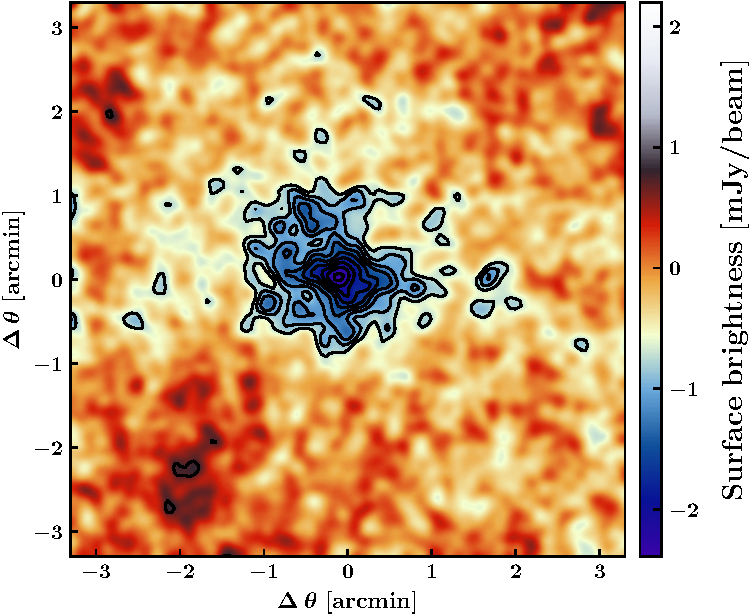
\includegraphics[height=6.6cm]{NIKA2_relax_map.pdf}
\hspace{1.2cm}
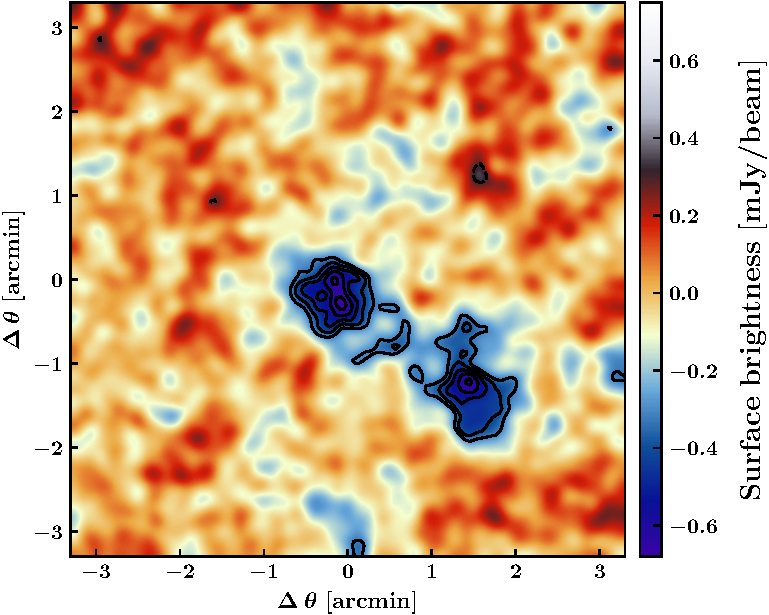
\includegraphics[height=6.6cm]{NIKA2_disturb_map.pdf}
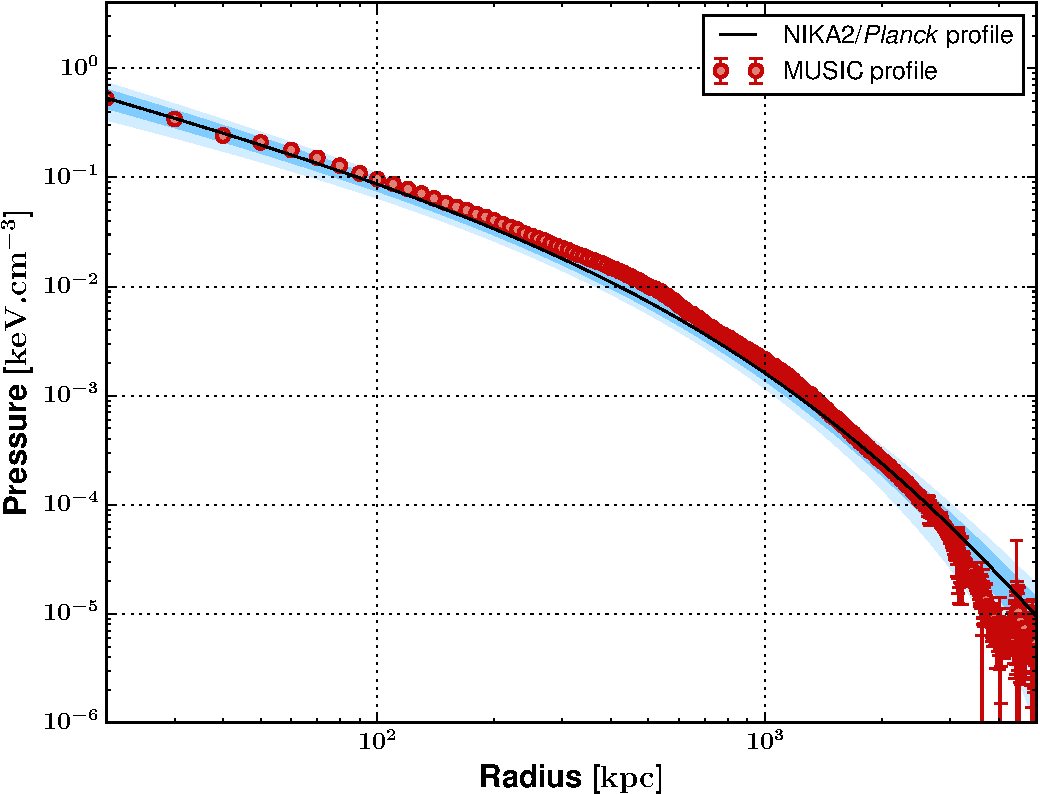
\includegraphics[height=6.6cm]{NIKA2_relax_profile.pdf}
\hspace{0.6cm}
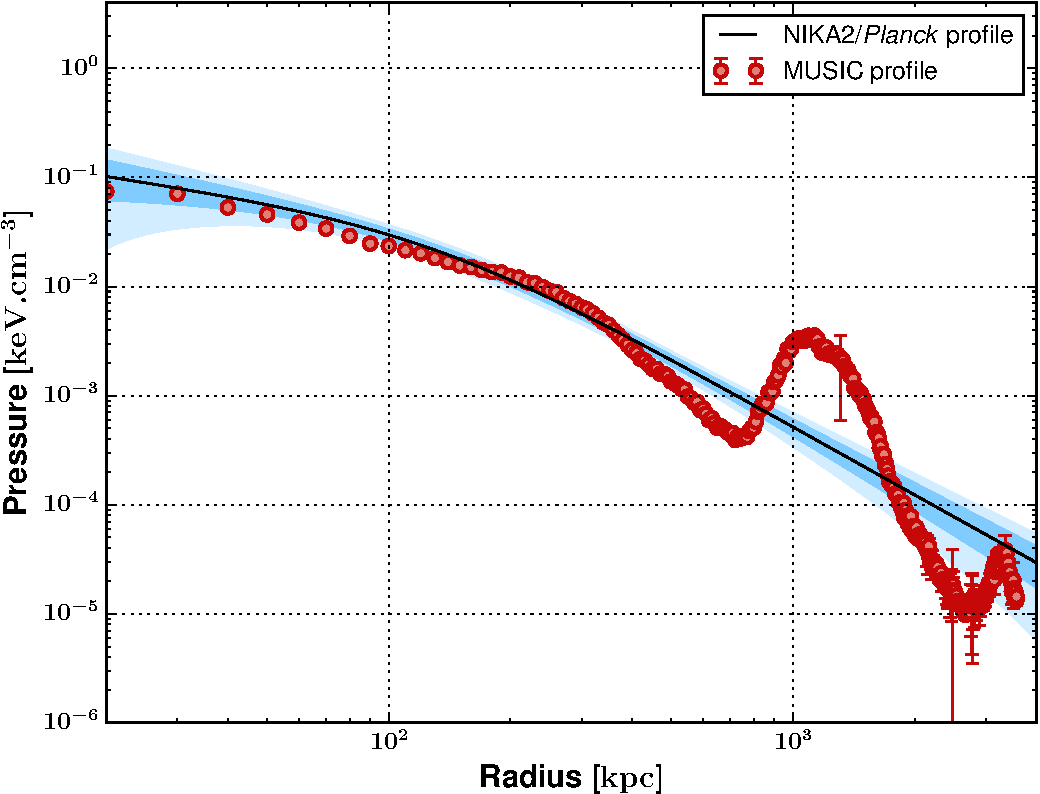
\includegraphics[height=6.6cm]{NIKA2_dist_profile.pdf}
\caption{{\footnotesize \textbf{Top:} Simulated NIKA2 tSZ surface brightness maps for a relaxed (left) and a disturbed (right) cluster. \textbf{Bottom:} Pressure profiles estimated at the maximum likelihood from the MCMC analysis based on the maps shown in the above panels (black line) and associated 1 and $2\sigma$ uncertainties (dark blue and light blue regions). The pressure profiles extracted from the MUSIC simulation for each cluster are represented by the red dots.}}
\label{fig:results_relax_disturbed}
\end{figure*}

The simulated NIKA2 and \planck\ tSZ maps are analyzed jointly using the NIKA2 tSZ analysis pipeline based on the MCMC procedure described in details in \citep{rup18}. We remind the main steps of the analysis here for the reader's convenience. The pressure distribution within the ICM of each selected MUSIC cluster is modeled by a gNFW pressure profile given the results obtained in Sect. \ref{subsec:music_prof}. At each iteration of the MCMC algorithm, a new set of gNFW profile parameters is generated. The pressure distribution is integrated along the line of sight in order to compute a model of the Compton parameter profile of the considered cluster (see eq. \ref{eq:y_compton}). The Compton parameter profile is then convolved with the beam profile of NIKA2 modeled as a two dimensional Gaussian function with a 17.7~arcsec FWHM. The convolved profile is then projected on the pixelized grid considered for the NIKA2 simulated data. We apply the NIKA2 transfer function to the computed Compton parameter map in order to account for the processing filtering that suppresses signal on large scales. The filtered Compton parameter map is converted into a NIKA2 tSZ surface brightness map using a conversion coefficient obtained by integrating the tSZ spectrum within the 150 GHz NIKA2 bandpass and by considering the temperature profile computed from the combination of the current pressure profile and the density profile extracted from the MUSIC simulation for the relativistic corrections.\\
As almost all the scales of the spatial distribution of the tSZ signal are smoothed by the \planck\ beam, we use the tSZ flux $Y_{\mathrm{5R500}}$ estimated by aperture photometry on the simulated \planck\ maps to average the information contained in all the pixels of each \planck\ map in a single measurement point. The model of the integrated Compton parameter is given by the spherical integral of the current pressure profile up to $5R_{500}$. The NIKA2 tSZ map model $\tilde{M}$ and the \planck\ integrated Compton parameter model $\tilde{Y}$ are then compared with the NIKA2 mock data $M_{\mathrm{NIKA2}}$ and the tSZ flux measured on the simulated \planck\ map using the following likelihood function:
\begin{equation}
\begin{tabular}{rl}
        $-2 \mathrm{ln} \, \mathscr{L}$  & $ =\chi^2_{\mathrm{NIKA2}} + \chi^2_{\mathrm{Planck}}$\\[0.2cm]
         &$ =\sum_{i=1}^{N_{\mathrm{pixels}}^{\mathrm{NIKA2}}} [(M_{\mathrm{NIKA2}} - \tilde{M})^T C_{\mathrm{NIKA2}}^{-1} (M_{\mathrm{NIKA2}} - \tilde{M})]_i $ \\[0.2cm]
         & $ + \left[\frac{Y_{\mathrm{5R500}} - \tilde{Y}}{\Delta Y_{\mathrm{5R500}}}\right]^2 $
\label{eq:chi2_NK2_Planck_MUSIC}
\end{tabular}
\end{equation}
where the uncertainty $\Delta Y_{\mathrm{5R500}}$ associated with the $Y_{\mathrm{5R500}}$ data point measured on the simulated \planck\ map corresponds to the dispersion of measurements performed around the cluster position where the noise is homogeneous. The NIKA2 correlated noise power spectrum considered to simulate the tSZ maps is used in order to estimate the noise covariance matrix $C_{\mathrm{NIKA2}}$ in the likelihood function (\ref{eq:chi2_NK2_Planck_MUSIC}). The MCMC analysis performed for each cluster is made by considering a total of 200 Markov chains on 20 CPUs in parallel. The convergence test of \cite{gel92} is used in order to stop the MCMC sampling of the parameter space. The computation time required for the latter to be completed is of the order of 2 to 3 days per cluster. At the end of each analysis the pressure profile obtained at the maximum likelihood is stored in a file along with the associated $1\sigma$ uncertainty on the pressure at each radius. The latter is estimated by Monte Carlo sampling of the posterior using the the Markov chains associated with each parameter of the gNFW model.\\

The maximum likelihood pressure profile is compared with the pressure profile extracted directly from the MUSIC simulation (see Sect. \ref{subsec:music_prof}). The left panels in Fig. \ref{fig:results_relax_disturbed} respectively present the simulated NIKA2 tSZ surface brightness map for a relaxed cluster of the penultimate mass bin of the low redshift bin (top) and its associated pressure profile (bottom). The black curve corresponds to the pressure profile obtained at the maximum likelihood and the uncertainties at 1 and $2\sigma$ are given by the dark and light blue regions. The red dots correspond to the pressure profile extracted from the MUSIC simulation for this cluster. The profile constrained by the MCMC analysis using a deprojection of the tSZ signal contained in the NIKA2 and \planck\ simulated maps is therefore compatible with the radial pressure distribution of the considered MUSIC cluster. This validates the procedure used in the NIKA2 tSZ analysis pipeline in order to estimate the pressure distribution of galaxy clusters from the combination of complementary tSZ data sets.\\

\begin{figure*}[h!]
\centering
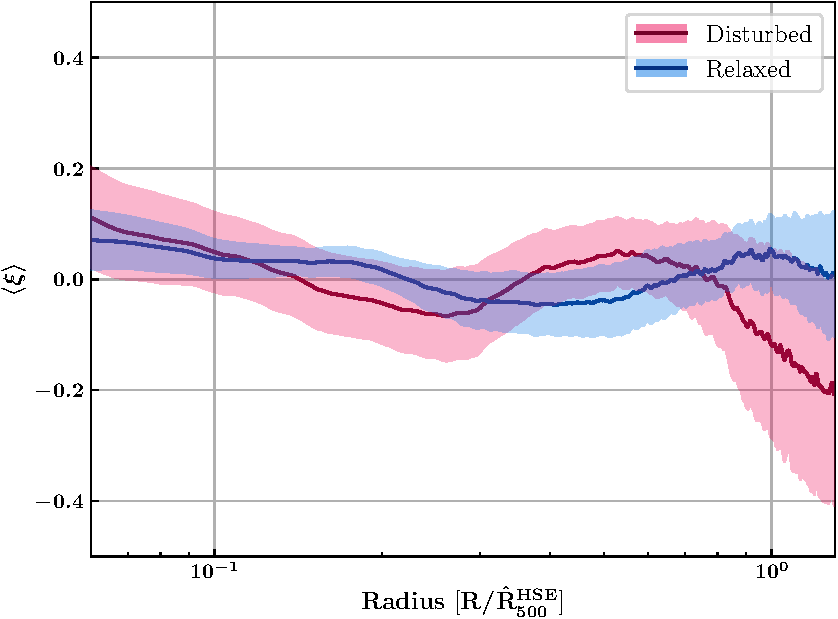
\includegraphics[height=6.4cm]{Estimation_error.pdf}
\hspace{0.6cm}
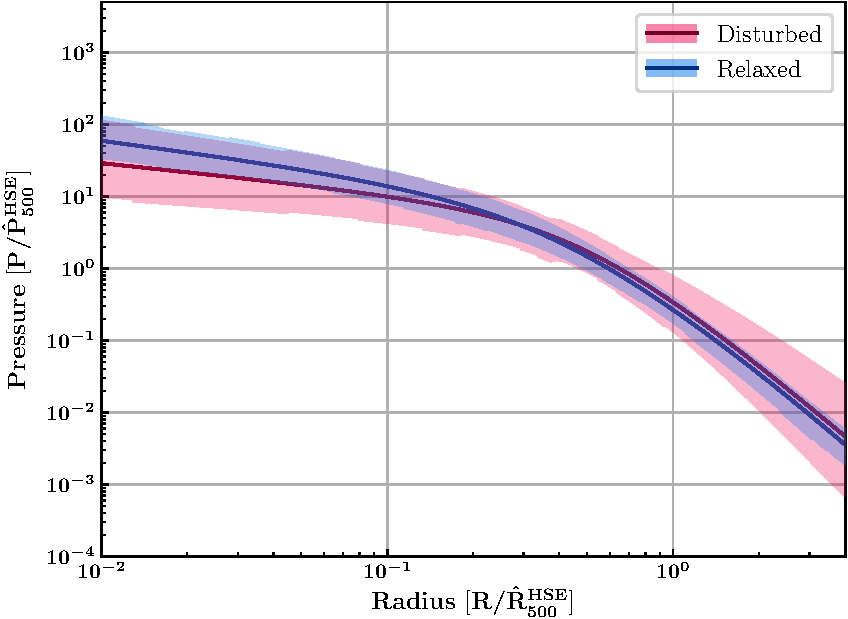
\includegraphics[height=6.4cm]{NIKA2_universals.pdf}
\caption{{\footnotesize \textbf{Left:} Mean relative errors as a function of the normalized radius between the NIKA2/\planck\ deprojected pressure profiles and the ones extracted from the MUSIC simulation for the relaxed (blue) and the disturbed (red) cluster samples. The shaded regions represent the $1\sigma$ error on the mean. \textbf{Right:} Mean normalized pressure profiles and associated scatter obtained from the profile distributions of relaxed (blue) and disturbed (red) clusters.}}
\label{fig:mean_pressure_prof}
\end{figure*}

The right panels in Fig. \ref{fig:results_relax_disturbed} correspond to the tSZ surface brightness map of a morphologically disturbed cluster of the second mass bin in the second redshift bin (top) and its associated pressure profile (bottom). Since this cluster is clearly bimodal and in a pre-merger state in the NIKA2 simulated map, a single gNFW model does not allow us to constrain all the features of the ICM radial pressure distribution extracted from the MUSIC simulation. As shown by the comparison between the profile obtained at the maximum likelihood and the profile extracted from the MUSIC simulation, the pressure distribution estimated from the MCMC analysis is significantly different from the mean radial distribution obtained in spherical shells for radii between 700 and 1500~kpc. Although the use of a non-parametric profile would enable constraining part of this deviation from the decreasing shape of the gNFW model, it is important to note that any model based on a radial pressure distribution is not suitable for this particular cluster because the circular symmetry of the spatial distribution of the tSZ signal is broken. A way to take this modelling error into account would be to mask the identified substructures of the disturbed clusters and perform the same analysis for each of them in order to estimate an additional systematic uncertainty on the estimated pressure profile. This type of analysis will be carried out for the clusters of the NIKA2 SZ large program but is beyond the scope of this study. We also note that the pressure profile estimated from the simulated tSZ observations of this cluster leads to a relative difference on the measurement of $\hat{Y}_{500}^{\mathrm{HSE}}$ of 67\% compared to the expected value obtained by considering the \cite{arn10} universal pressure profile and the measurement of $\hat{Y}_{\mathrm{5R500}}$ computed by aperture photometry on the simulated \planck\ map. This highlights the impact of the NIKA2 high angular resolution on the estimation of the integrated parameter of high redshift clusters.\\

At the end of the MCMC analysis of each simulated tSZ map, the constrained pressure profile is combined with the density profile extracted from the MUSIC simulation\footnote{We treat the latter as a density profile estimated by X-ray observations.} in order to estimate a mass profile under the hydrostatic equilibrium hypothesis using eq. (\ref{eq:mass_HSE}). The latter is used in order to compute the value of the characteristic radius $\hat{R}_{500}^{\mathrm{HSE}}$ considered to estimate the integrated quantities $\hat{M}_{500}^{\mathrm{HSE}}$, $\hat{Y}_{500}^{\mathrm{500}}$ and $\hat{P}_{500}^{\mathrm{HSE}}$ (see Sect. \ref{subsec:music_integ}). These quantities are essential to estimate the mean pressure profile from all the pressure profiles obtained by this analysis.

\subsection{Impact of the ICM dynamical state on the mean pressure profile}\label{subsec:impact_icm_dist}

This section is dedicated to the analysis of the impact of the ICM dynamical state  of the selected MUSIC clusters on the individual pressure profiles estimated from the analysis developed in Sect. \ref{subsec:profile_extract} and on the mean pressure profile of the relaxed and disturbed cluster samples.\\
The pressure profiles estimated at the end of the analysis described in Sect. \ref{subsec:profile_extract} are normalized using the values of $\hat{R}_{500}^{\mathrm{HSE}}$ and $\hat{P}_{500}^{\mathrm{HSE}}$ computed for each cluster by the combination of the MUSIC density profile and the NIKA2/\planck\ deprojected pressure profile. As the uncertainties associated with the estimated pressure profiles for the disturbed clusters do not reflect the true errors made on the characterization of the pressure distribution of these clusters (see Sect. \ref{subsec:profile_extract}), we decide to compare the estimated pressure profiles $\tilde{P}$ with the MUSIC profiles extracted from the simulation $P_{\mathrm{MUSIC}}$ by computing the relative error,
\begin{equation}
\xi = \frac{P_{\mathrm{MUSIC}} - \tilde{P}}{P_{\mathrm{MUSIC}}}
\end{equation}
The variations of $\xi$ as a function of $R/\hat{R}_{500}^{\mathrm{HSE}}$ for all the selected MUSIC clusters are then used to compute the mean and the error on the mean of the distributions of $\xi$ measured at each scaled radius for the disturbed and the relaxed clusters. The left panel of Fig. \ref{fig:mean_pressure_prof} shows the variations of the mean value of $\xi$ as a function of the normalized radius $R/\hat{R}_{500}^{\mathrm{HSE}}$ for the relaxed (blue) and disturbed (red) simulated clusters. The shaded blue and red regions give the $1\sigma$ errors on the mean values of $\xi$ computed at each radius as the standard deviation of the distributions divided by the square root of the number of relaxed and disturbed profiles respectively. The relative error between the deprojected pressure profile and the one extracted in the three dimensional volume of the simulation is always lower than 10\% in the radius range where the tSZ signal is not filtered significantly by NIKA2, \emph{i.e.} for $R$ between $0.1 \, \hat{R}_{500}^{\mathrm{HSE}}$ and $\hat{R}_{500}^{\mathrm{HSE}}$. Furthermore, the average of the mean relative error in this radius range is equal to 0.9\% and 0.05\% for the disturbed and the relaxed clusters respectively. The variations of $\xi$ around 0 are due to deviations of the shape of the simple gNFW model from the true pressure distribution of the simulated clusters. Although these deviations tend to be small for relaxed clusters (see the left panels of Fig. \ref{fig:results_relax_disturbed}), they can reach an order of magnitude at specific radii for disturbed systems (see the right panels of Fig. \ref{fig:results_relax_disturbed}). This explains why the error on the mean of $\xi$ associated with the disturbed clusters is on average 90\% larger than the one measured for the relaxed clusters. We note however that the mean relative error computed for the disturbed clusters in the radius range of interest for NIKA2 is not significantly larger than the one measured for the relaxed clusters. This comes from the fact that the location of unvirialized structures in the ICM of the disturbed clusters is not always the same. The large relative errors measured in a given radius range thus tend to compensate each others for a sample of disturbed systems. This implies that the mean normalized pressure profiles obtained by analyzing the simulated NIKA2 and \planck\ data for the two sub-samples are compatible with the mean profiles obtained by combining the profiles extracted from the MUSIC simulation for the selected clusters.\\

The distribution of the normalized pressure profiles for the relaxed and disturbed selected clusters are treated separately in order to estimate the mean pressure profile associated with the two populations at high redshift using the method developed in the Sect. \ref{subsec:music_prof}. The pressure values in each profile are weighted by their associated error bars in the calculation of the mean profile (see Sect. \ref{subsec:profile_extract}). The resulting mean profiles are represented with the blue and red lines in the right panel of Fig. \ref{fig:mean_pressure_prof}. The blue and red shaded regions represent the scatter of the distributions of normalized pressure profiles for the relaxed and disturbed clusters respectively. The flattening of the mean pressure profile associated with the disturbed clusters in the core of the ICM compared to the profile associated with the relaxed clusters is consistent with the trend observed in different observational studies \citep[\emph{e.g.}][]{arn10}. The scatter associated with the mean profiles in the central region of the clusters ($r < 0.1\mathrm{R_{500}}$) and their outskirts ($r > 2\mathrm{R_{500}}$) are about 20 and 30\% higher than those associated with the mean profiles estimated from the MUSIC profiles for the relaxed and disturbed clusters respectively. The increase of the scatter observed for the relaxed clusters is due to the angular resolution of NIKA2 at 150~GHz and its finite field of view, that do not allow the central parts of high redshift clusters to be resolved and their outskirt to be mapped without significant filtering. For disturbed clusters, the observed increase of the scatter is more significant, especially in the outskirt, because the constraints on the external slopes of the individual profiles are affected by the presence of substructures and deviations from circular symmetry. The scatter associated with the mean profile of the disturbed clusters is 65\% greater than the one observed for the profile distribution of the relaxed clusters at a radius $R = \mathrm{R_{500}}$. This result shows the importance of the NIKA2 high-resolution tSZ observations in order to accurately measure the fraction of disturbed clusters at high redshift and therefore the true intrinsic scatter associated with the mean pressure profile of a representative cluster sample at $0.5 < z < 0.9$. Indeed, this study shows that the instrumental characteristics of the NIKA2 camera enable discriminating relaxed and disturbed ICM regions in a simulated sample of galaxy clusters similar to the one considered for the NIKA2 SZ large program. The latter will therefore enable characterizing the impact of the detected ICM disturbances on the mean pressure profile obtained under the hypothesis of the spherical cluster in hydrostatic equilibrium.

\section{Conclusions}\label{sec:Conclusions}

We have used synthetic clusters from the MUSIC simulation in order to build a sample of realistic NIKA2 and \planck\ simulated tSZ observations similar to the ones that will be obtained with the NIKA2 SZ large program. These mock observations have been used jointly in the NIKA2 SZ pipeline in order to estimate the pressure profile of each selected cluster under the hypothesis of the spherical cluster in hydrostatic equilibrium. The deprojected profiles have been used in order to estimate the mean normalized pressure profiles associated with the samples of relaxed and disturbed selected clusters.\\

The instrumental characteristics of NIKA2 and \planck\ enable identifying a significant impact of the ICM dynamical state on the characterization of the mean normalized pressure profile used in cosmological analyses. More particularly, we have shown that it is essential to accurately characterize the fraction of disturbed clusters in a representative sample of high redshift galaxy clusters in order to estimate the intrinsic scatter associated with the mean normalized pressure profile and the value of the central slope of the latter. If the self-similar hypothesis of cluster formation is not verified at high redshift, it will be essential to consider the intrinsic properties of the distributions of normalized pressure profiles, estimated on cluster samples in restricted mass and redshift ranges, in order to minimize the bias associated with the pressure profile evolution on the constraints of cosmological parameters.\\

The NIKA2 SZ large program will elucidate the origin and the impact of high redshift ICM disturbances on the scatter of the pressure profile distribution. The high angular resolution of NIKA2 will be used in order to estimate the fraction of disturbed clusters in a representative sample of galaxy clusters at redshifts $0.5<z<0.9$ and study its evolution with redshift. This task will not be trivial because it is challenging to define reliable morphological indicators that clearly separate relaxed and disturbed cluster populations from tSZ maps only. It will be necessary to combine morphological indicators specific to the X-ray maps of \xmm\ and the tSZ maps of NIKA2 in order to improve the criteria currently used to characterize the morphology of galaxy clusters. These joint analyses will benefit from the different dependencies of these observables on the thermodynamic properties of the ICM and their integral along the line of sight. The combination of NIKA2 and \xmm\ observations will also enable estimating a potential deviation from the self-similar cluster formation processes by comparing the products of the NIKA2 SZ large programme with the tSZ results obtained by other low redshift studies (\emph{e.g.} \citep{pla13}). These results will therefore contribute to the understanding of the potential tension currently observed between the different estimates of the $\sigma_8$ and $\Omega_m$ parameters.

%###############################################################################################
%##########################                       ACKNOWLEDGEMENTS                        ##########################%###############################################################################################
\begin{acknowledgements}
We would like to thank the IRAM staff for their support during the campaigns and the anonymous referee for helpful comments. 
The NIKA dilution cryostat has been designed and built at the Institut N\'eel. 
In particular, we acknowledge the crucial contribution of the Cryogenics Group, and 
in particular Gregory Garde, Henri Rodenas, Jean Paul Leggeri, and Philippe Camus. 
This work has been partially funded by the Foundation Nanoscience Grenoble, the LabEx FOCUS ANR-11-LABX-0013, and 
the ANR under the contracts "MKIDS", "NIKA", and ANR-15-CE31-0017. This work has benefited from the support of the European Research Council Advanced Grants ORISTARS and M2C under the European Union’s Seventh Framework Programme (Grant Agreement Nos. 291294 and 340519). Support for this work was provided by NASA through SAO Award Number SV2-82023 issued by the Chandra X-Ray Observatory Center, which is operated by the Smithsonian Astrophysical Observatory for and on behalf of NASA under contract NAS8-03060. We acknowledge funding from the ENIGMASS French LabEx (R. A. and F. R.), 
the CNES post-doctoral fellowship program (R. A.),  the CNES doctoral fellowship program (A. R.), and 
the FOCUS French LabEx doctoral fellowship program (A. R.). R.A. acknowledges support from the Spanish Ministerio de Econom\'ia and Competitividad (MINECO) through grant number AYA2015-66211-C2-2.
\end{acknowledgements}

\begin{thebibliography}{81}
\expandafter\ifx\csname natexlab\endcsname\relax\def\natexlab#1{#1}\fi

\bibitem[{Adam \emph{et~al.}(2014)}]{ada14}
Adam, R., {et~al.} 2014, \aap, \textbf{569}, A66

\bibitem[{Adam \emph{et~al.}(2015)}]{ada15}
Adam, R., {et~al.} 2015, \aap, \textbf{576}, A12

 \bibitem[{Adam \emph{et~al.}(2016)}]{ada16a}
Adam, R., Comis, B., Bartalucci, I., \emph{et~al.} 2016, \aap, \textbf{586}, A122

\bibitem[{Adam \emph{et~al.}(2017{\natexlab{a}})}]{ada17a}
Adam, R., Bartalucci, I., Pratt, G. W., \emph{et~al.} 2017{\natexlab{a}}, \aap, \textbf{598}, A115

\bibitem[{Adam \emph{et~al.}(2017{\natexlab{b}})}]{ada17b}
Adam, R., Arnaud, M., Bartalucci, I., \emph{et~al.} 2017{\natexlab{b}}, \aap, \textbf{606}, A64

\bibitem[{Adam \emph{et~al.}(2018)}]{ada18}
Adam, R., Adane, A., Ade, P.A.R, \emph{et~al.} 2018, \aap, \textbf{609}, A115

\bibitem[{{Anderson} \emph{et~al.}(2014)}]{and14}
{Anderson}, L., {Aubourg}, E., {Bailey}, S., \emph{et~al.} 2014, \mnras, \textbf{441}, 24

\bibitem[{Arnaud \emph{et~al.}(2010)}]{arn10}
Arnaud, M., Pratt, G.~W., Piffaretti, R., \emph{et~al.}, 2010, \aap, \textbf{517}, A92

\bibitem[{Birkinshaw(1999)}]{bir99}
Birkinshaw, M. 1999, Phys. Rept., \textbf{310}, 97

\bibitem[{{B{\"o}hringer} \emph{et~al.}(2016)}]{boe16}
B{\"o}hringer, H., \& Chon, G., 2016, Mod. Phys. Lett., \textbf{31}, 1640008

\bibitem[{Bolliet \emph{et~al.}(2018)}]{bol18}
Bolliet, B., Comis, B., Komatsu, E., \& Macías-Pérez J. F. 2018, \mnras, \textbf{477}, 4957–4967

\bibitem[{Borgani \emph{et~al.}(2011)}]{bor11}
Borgani, S., \& Kravtsov 2011,  Advanced Science Letters, \textbf{4}, 204–227

\bibitem[{Bourrion \emph{et~al.}(2016)}]{bou16}
Bourrion, O., Benoit, A., Bouly, J. L., \emph{et~al.} 2016, J. Instrum., \textbf{11}, P11001

\bibitem[{Calvo \emph{et~al.}(2016)}]{cal16}
Calvo, M., Benoit, A., Catalano, A., \emph{et~al.}  2016, J. Low Temp. Phys., \textbf{184}, 816

\bibitem[{Carlstrom \emph{et~al.}(2002)Carlstrom, Holder, \& Reese}]{car02}
Carlstrom, J.~E., Holder, G.~P., \& Reese, E.~D. 2002, \araa, \textbf{40}, 643


\bibitem[{{Cialone} \emph{et~al.}(2018)}]{cia18}
{Cialone}, G., De Petris, M., Sembolini, F., \emph{et~al.} 2018, \mnras, \textbf{477}, 139–152

\bibitem[{Comis \emph{et~al.}(2016)}]{com16}
Comis, B., {et~al.} 2016, in {51st Rencontres de Moriond on Cosmology La
  Thuile, Italy, March 19-26, 2016}, 1605.09549

\bibitem[{Dicker \emph{et~al.}(2014)}]{dic14}
Dicker, S. R., \emph{et~al.} 2014, SPIE Conference Series, \textbf{9153}, 0

\bibitem[{{Dolag} \emph{et~al.}(2008)}]{dol08}
{Dolag}, K., Borgani, S., Schindler, S., \emph{et~al.} 2008, Space Science Reviews, \textbf{134}, 229-268

\bibitem[{Gelman \& Rubin(1992)}]{gel92}
Gelman, A., \& Rubin, D.~B. 1992, Statist. Sci., \textbf{7}, 457

\bibitem[{Hilton \emph{et~al.}(2018)}]{hil18}
Hilton, M., Hasselfield, M., Sif\'on, C., \emph{et~al.} 2018, Accepted for publication in ApJS, 1709.05600

\bibitem[{Itoh \emph{et~al.}(1998)Itoh, Kohyama, \& Nozawa}]{ito98}
Itoh, N., Kohyama, Y., \& Nozawa, S. 1998, \apj, \textbf{502}, 7

\bibitem[{Kitayama \emph{et~al.}(2016)}]{kit16}
Kitayama, T., Ueda, S., Takakuwa, S., \emph{et~al.} 2016, Publications of the Astronomical Society of Japan, \textbf{68}, 88

\bibitem[{{Klypin} \emph{et~al.}(2001)}]{kly01}
{Klypin}, A., Kravtsov, A. V., Bullock, J., \& Primack, J. 2001, \apj, \textbf{554}, 903-915

\bibitem[{{Komatsu} \emph{et~al.}(2011)}]{kom11}
{Komatsu}, E., Smith, K. M., Dunkley, J., \emph{et~al.} 2011, \apjs, \textbf{192}, 18

\bibitem[{{von der Linden} \emph{et~al.}(2014)}]{lin14}
{von der Linden}, A., Allen, M. T., Applegate, D. E., \emph{et~al.} 2014, \mnras, \textbf{439}, 2

\bibitem[{Melin \emph{et~al.}(2006)}]{mel06}
{Melin}, J.-B., {Bartlett}, J. G., Delabrouille, J., \emph{et~al.} 2006, \aap, \textbf{459}, 341 - 352

\bibitem[{Monfardini \emph{et~al.}(2010)}]{mon10}
Monfardini, A., Swenson, L. J., Bideaud, A., \emph{et~al.} 2010, \aap, \textbf{521}, A29

\bibitem[{Mroczkowski \emph{et~al.}(2018)}]{mro18}
Mroczkowski, T., Nagai, D., Basu, K., \emph{et~al.} 2018, Submitted to Space Science Reviews, 1811.02310

\bibitem[{{Nagai} \emph{et~al.}(2007)}]{nag07}
{Nagai}, D., {Kravtsov}, A.~V., \& {Vikhlinin}, A. 2007, \apj, \textbf{668}, 1

\bibitem[{{Planck Collaboration} \emph{et~al.}(2013)}]{pla13}
{Planck Collaboration}, \emph{et~al.} 2013, \aap, \textbf{550}, A133

\bibitem[{{Planck Collaboration} \emph{et~al.}(2014)}]{pla14}
{Planck Collaboration}, \emph{et~al.} 2014, \aap, \textbf{571}, A20

\bibitem[{{Planck Collaboration} \emph{et~al.}(2016{\natexlab{a}})}]{pla16a}
{Planck Collaboration}, \emph{et~al.} 2016{\natexlab{a}}, \aap, \textbf{594}, A24

 \bibitem[{{Planck Collaboration} \emph{et~al.}(2016{\natexlab{b}})}]{pla16b}
{Planck Collaboration}, \emph{et~al.} 2016{\natexlab{b}}, \aap, \textbf{594}, A27

\bibitem[{{Planck Collaboration} \emph{et~al.}(2018)}]{pla18}
{Planck Collaboration}, \emph{et~al.} 2018, 1807.06209

\bibitem[{Perlmutter \emph{et~al.}(1997)}]{per97}
Perlmutter, S., Aldering, G., Deustua, S., \emph{et~al.} 1997, Bull. Am. Astron. Soc., \textbf{29}, 1351

\bibitem[{Pointecouteau \emph{et~al.}(1998)}]{poi98}
Pointecouteau, E., Giard, M., \& Barret, D. 1998, \aap, \textbf{336}, 44

\bibitem[{{Prada} \emph{et~al.}(2012)}]{pra12}
{Prada}, F., Klypin, A. A., Cuesta, A. J., \emph{et~al.} 2012, \mnras, \textbf{423}, 3018–3030

\bibitem[{Roesch \emph{et~al.}(2012)}]{roe12}
Roesch, M., Benoit, A., Bideaud, A., \emph{et~al.} 2012, ISSTT2011 Workshop, 1212.4585

\bibitem[{Romero \emph{et~al.}(2017)}]{rom17}
Romero, C., McWilliam, M., Mac\'ias-P\'erez, J. F., \emph{et~al.} 2017, submitted to \aap, 1707.06113

\bibitem[{Rossetti \emph{et~al.}(2017)}]{ros17}
Rossetti, M., Gastaldello, F., Eckert, D., 2017, \mnras, \textbf{468}, 1917–1930
  
 \bibitem[{Ruppin \emph{et~al.}(2017)}]{rup17}
Ruppin, F., Adam, R., Comis, B., \emph{et~al.} 2017, \aap, \textbf{597}, A110

 \bibitem[{Ruppin \emph{et~al.}(2018)}]{rup18}
Ruppin, F., Mayet, F., Pratt, G.~W., \emph{et~al.} 2018, \aap, \textbf{615}, A112

\bibitem[{Salvati \emph{et~al.}(2018)}]{sal18}
{Salvati}, L., {Douspis}, M., {Aghanim}, N., \emph{et~al.} 2018, \aap, \textbf{614}, A13

\bibitem[{Sembolini \emph{et~al.}(2012)}]{sem12}
Sembolini, F., Yepes, G., De Petris, M., \emph{et~al.}, 2012, \mnras, \textbf{429}, 323-343

 \bibitem[{Shaw  \emph{et~al.}(2008)}]{sha08}
Shaw, L. D., Holder, G. P., \& Bode, P. 2008, \apj, \textbf{686}, 1
 
\bibitem[{{Springel} \emph{et~al.}(2001)}]{spr01}
{Springel}, V., Yoshida , N., \& White , S. D. M. 2001, New Astronomy, \textbf{6}, 79

\bibitem[{{Springel} \& Hernquist(2003)}]{spr03}
{Springel}, V., \& Hernquist, L., 2003, \mnras, \textbf{339}, 289
  
\bibitem[{Sunyaev \& Zeldovich(1972)}]{sun72}
Sunyaev, R.~A., \& Zeldovich, Y.~B. 1972, Comments on Astrophysics and Space
  Physics, \textbf{4}, 173
  
  \bibitem[{Sunyaev \& Zeldovich(1980)}]{sun80}
Sunyaev, R.~A., \& Zeldovich, {\relax Ya}.~B. 1980, \araa, \textbf{18}, 537

\bibitem[{Tinker \emph{et~al.}(2008)}]{tin08}
{Tinker}, J., {Kravtsov}, A. V., {Klypin}, A., \emph{et~al.} 2008, \apj, \textbf{688}, 2

\bibitem[{Voit (2005)}]{voi05}
Voit, M., 2005, Rev. Mod. Phys., \textbf{77}, 207-258

\end{thebibliography}

\end{document}
